\chapter{Machine Learning}\label{neural-network---practical-lesson-8}

In this Chapter we will see how machine learning techniques can be
successfully applied to solve financial problems. We will first do a
quick tour on the theory behind neural networks and then we will see an
example and two practical applications regarding regression and
classification issues.

This lecture just scratches the surface of the
machine learning topic which has seen a huge development in the latest
years leading to thousands of applications in many different fields.
    
\section{Neural Networks}\label{neural-networks}

Artificial Neural Networks (ANN or simply NN) are information processing
models that are developed by inspiring from the working principles of
human brain. Their most essential property is the ability of learning
from sample sets.

The basic unit of ANN architecture are neurons which internally may be in
connection with other neurons.

\begin{figure}[htb]
	\centering
	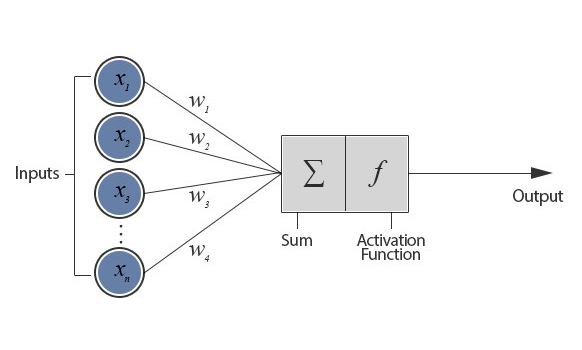
\includegraphics[width=0.7\textwidth]{figures/neuron}
	\caption{Model of an artificial neuron.}
        \label{fig:neuron}
\end{figure}

A neuron consists of weights (\(w_i\)) and real numbers (\(x_i\)). All
inputs injected into a neuron are individually weighted, added together
(sometimes it is added also a bias \(w_0\)) and passed into the
activation function which produce the neuron output

\[ \textrm{Inputs} = \sum_{i=1}^{N} x_i w_i +w_0 \rightarrow f(\textrm{Inputs}) = \textrm{Outputs}\]

Figure~\ref{fig:neuron} shows an example.
There are many different types of activation function and two of the simpler are the \emph{step function},
which returns just 0 or 1 according
to the input value, and the \emph{sigmoid} which can be thought
of as the continuous version of the step function, see Fig.~\ref{fig:sigmoid}.

\begin{figure}[htb]
	\centering
	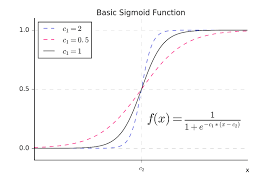
\includegraphics{figures/sigmoid.png}
	\caption{Sigmoidal activation function.}
        \label{fig:sigmoid}
\end{figure}

Other commonly used activation functions are the \emph{Rectified Linear Unit}
(ReLU) and the \emph{hyperbolic tangent} (tanh).

For an deeper discussion of activation functions see
\href{https://medium.com/the-theory-of-everything/understanding-activation-functions-in-neural-networks-9491262884e0}{this article}

\subsection{Training of a Neuron}\label{training-of-a-neuron}

When teaching children how to recognize a bus, we just tell them,
showing an example: "This is a bus. That is not a bus." until they
learn the concept of what a bus is. Furthermore, if the child sees new
objects that she hasn't seen before, we could expect her to recognize
correctly whether the new object is a bus or not.

This is exactly the idea behind neurons. Similarly, inputs from a
\emph{training} set are presented to the neuron one after the other
together with the correct output and the neuron weights are modified
accordingly.

When an entire pass through all of the input training vectors is
completed (\emph{epoch}) the neuron has learnt ! (to make it learn better
training data can be processed multiple times)

At this time, if an input vector \(\mathbf{x}\) (already in the training
set) is given to the neuron, it will output the correct value. If
\(\mathbf{x}\) is not in the training set, the network will respond with
an output similar to other training vectors close to \(\mathbf{x}\).

This kind of training is called \emph{supervised} because we have a set of training data with known targets and, during training, we want our model to learn to predict the target from the other variables.

Unfortunately using just a neuron is not too useful since it is not
possible to solve the interesting problems we would like to face with
just that simple architecture. The next step is then to put together
more neurons in \emph{layers}.

\subsection{Multilayered Neural Networks}\label{multi-layered-neural-networks}

\begin{figure}[htb]
	\centering
	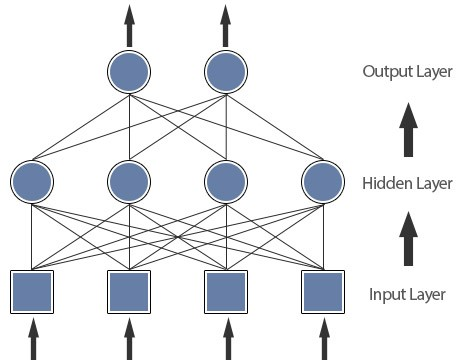
\includegraphics[width=0.7\textwidth]{figures/multilayer.jpeg}
	\caption{A multi-layered neural network.}
        \label{fig:multilayered_nn}
\end{figure}

Each input from the \emph{input layer} is fed up to each node in the
next hidden layer, and from there to each node on the output layer. We
should note that there can be any number of nodes per layer and there
are usually multiple hidden layers to pass through before ultimately
reaching the output layer. Figure~\ref{fig:multilayered_nn} shows a simple
example of such architecture.

\subsection{Training a Multilayered Neural Network}\label{training-a-multilayered-neural-network}

The training of a multilayered NN follows these steps:

\begin{itemize}
	\tightlist
	\item
	present a training sample to the neural network (initialized with
	random weights);
	\item
	compute the network output obtained by calculating activation functions of each layer;
	\item
	calculate the error (loss) as the difference between the NN predicted
	output and the actual output;
	\item
	having calculated the error, re-adjust the weights of the network such
	that the error (difference) decreases;
	\item
	continue the process for all samples several times (epochs) until the
	weights are not changing too much (i.e. the process converged).
\end{itemize}

\begin{figure}[htb]
	\centering
	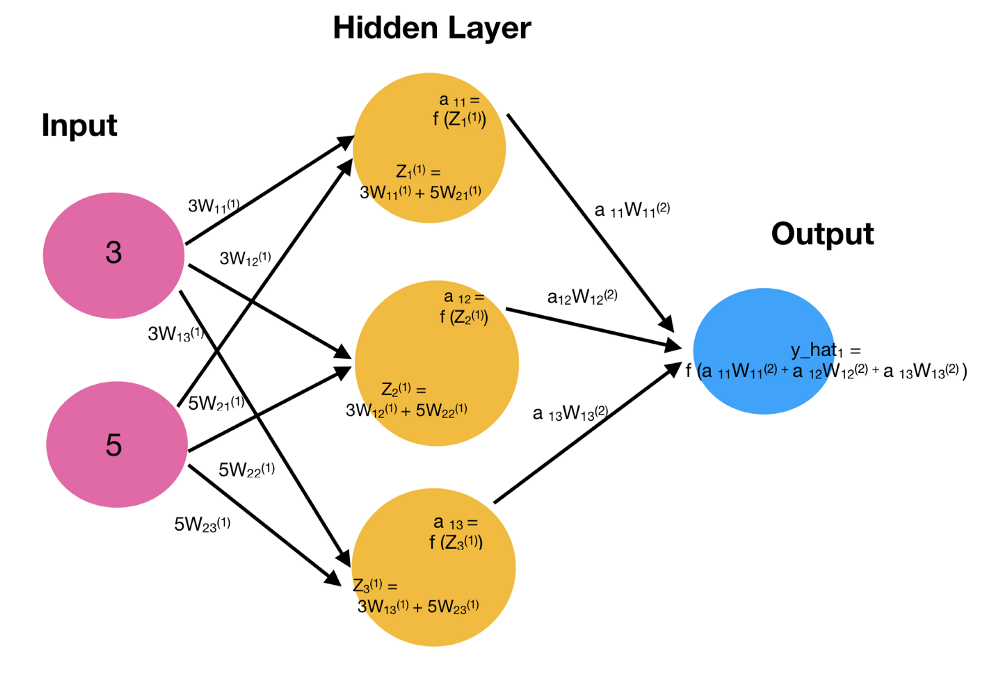
\includegraphics[width=0.7\textwidth]{figures/training_nn}
	\caption{Optimization of the weights done minimizing the loss function.}
        \label{fig:training}
\end{figure}

In Figure~\ref{fig:training} an example of training is shown.
The NN error is computed by the \emph{loss function}. Different loss
functions will give different errors for the same prediction, and thus
have a considerable effect on the performance of the model. Two are the
main possible choices

\begin{itemize}
	\tightlist
	\item
	Mean Absolute Error (MAE): the average of the absolute value of the
	differences between the predictions and true values;
	\item
	Root Mean Squared Error (MSE): the square root of the average of the
	squared differences between the predictions and true values.
\end{itemize}

The mean absolute error is easily interpretable, as it represents how
far off we are on average from the correct value. The root mean squared
error penalizes larger errors more heavily and is commonly used in
regression tasks. Either metrics may be appropriate depending on the
situation and you can use both for comparison.
\href{https://medium.com/human-in-a-machine-world/mae-and-rmse-which-metric-is-better-e60ac3bde13d}{Here}
is a discussion of the merits of these metrics.

The error or loss is a function of the internal parameters of the model
(i.e the weights and bias). For accurate predictions, one needs to
minimize the calculated error. In a neural network, this is done using
\emph{back propagation} (see
\href{https://towardsdatascience.com/understanding-backpropagation-algorithm-7bb3aa2f95fd}{this article}).
The current error is typically propagated backwards to previous layers,
where it is used to modify the weights and bias in such
a way that the error tends to be minimized.

The weights are modified using a function called Optimization Function
(we will use \emph{Adam} in the following but there are
more).

%\begin{figure}[htb]
%	\centering
%	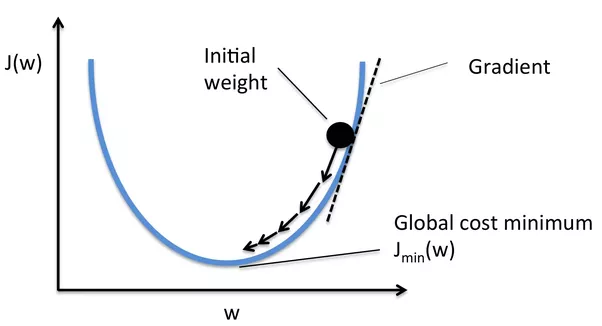
\includegraphics[width=0.7\textwidth]{figures/loss_function}
%	\caption{Optimization of the weights done minimizing the loss function.}
%\end{figure}

A common mistake to avoid is to \emph{overtrain} or \emph{overift} a NN. %Overtraining is  what happens when the NN learns too well the training sample but its performance degrade substantially in an independent testing sample.
Overfitting is when a model is trained too well on the training data. You want to avoid overfitting, as this would mean that the model mostly just memorized the training data. This would account for a large accuracy with the training data but a low accuracy in the testing data. 

At least it is required to split the available sample in two parts:
training and testing (e.g.~80\% and 20\%) and to use the former to
perform the training and the latter to cross-check the performance.
\textbf{Usually performance are measured using the loss function value
at the end of the training.}

Actually you should split the sample in three parts: training, testing and validation. What you would usually do is take the model with the highest validation accuracy and then test the model with the testing set.
%This makes sure that you don’t overfit the model. Using the validation set to choose the best model is a form of data leakage (or “cheating”) to get to pick the result that produced the best test score out of hundreds of them. Data leakage happens when information outside the training data set is used in the model.
In this case, our testing and validation set are the same, since we have a smaller sample size.

\subsection{Neural Network Design}\label{neural-network-design}

There is no rule to guide developer into the design of a neural network
in terms of number of layers and neuron per layer (the so called hyperparameters). 
One popular method for hyperparameter optimization is grid search. What this method does is it takes lists of parameters and it runs the model with each parameter combination that it can find. It is the most thorough way but also the most computationally heavy way to do this.

%The most common strategy is trail and error where you finally pick up the solution giving the best accuracy. In general a larger number of nodes is better to catch highly structured data with a lot of feature although it mayrequire larger training sample to work correctly.
Anyway as a rule of thumb a NN with just one hidden layer with a number
of neurons averaging the inputs and outputs is sufficient in most cases.

In the following we will use more complex networks just for
illustration, no strong attempt in optimizing the layout has been done
though.

\subsection{Regression and Classification}\label{regression-and-classification}

The two main categories of problems that can be solved with neural
networks are \emph{classification} and \emph{regression}. Let's see
their characteristics and differences.

\subsubsection{Classification}\label{classification}

Classification is a process of finding a function which helps in dividing
the dataset into classes based on different parameters. 
The task of the classification algorithm is to find the mapping function
to map the input (\(x\)) to the \textbf{discrete} output (\(y\)). We try
to find the decision boundary, which can divide the dataset into
different classes.

A typical example of classification problem is
\emph{email spam detection}. The model is trained on the basis of millions of
emails on different parameters, and whenever it receives a new email, it
identifies whether the email is spam or not. If the email is spam, then
it is moved to the spam folder. Classification algorithms can also be used in
speech recognition, car plates identification, etc.

\subsubsection{Regression}\label{regression}

Regression is the process of finding the correlations between dependent
and independent variables. It helps in predicting continuous
variables such as market trends, house prices, etc.

The task of the regression algorithm is to find the mapping function to
map the input variable (\(x\)) to the \textbf{continuous} output
variable (\(y\)), trying to find the best fit which can predict the
output more accurately.

As an example suppose we want to do weather forecasting, so for this, we will
use a regression algorithm. The model is trained
on past data, and once the training is completed, it can predict the
weather for future days. In general whenever we are dealing with
function approximation this kind of algorithms can be applied.

\subsubsection{Technical Note}\label{technical-note}

Neural network training and testing is performed using two modules:
\(\tt{keras}\) (which in turn is based on a Google open source library
called \(\tt{tensorflow}\)) and \(\tt{scikit-learn}\) which provide many
useful utilities.

In order hide as much as possible the many little details that have to
be set when developing NN I have developed a simple class
(\(\tt{FinNN}\)) which relies on \(\tt{keras}\) anyway but should make
the whole process easier.

\section{Function approximation}\label{function-approximation}

As a first practical example let's try to design an ANN which is capable
of learning the functional form underlying a set of data.

Let's generate a sample with \(x\) (input), \(f(x)\) (target output)
pairs where \(f(x) = x^3 +2\) and let's start to code the NN structure.

We start by importing the necessary modules.

\begin{tcolorbox}[breakable, size=fbox, boxrule=1pt, pad at break*=1mm,colback=cellbackground, colframe=cellborder]
\begin{Verbatim}[commandchars=\\\{\}]
\PY{k+kn}{from} \PY{n+nn}{finnn} \PY{k}{import} \PY{n}{FinNN}
\PY{k+kn}{import} \PY{n+nn}{numpy} \PY{k}{as} \PY{n+nn}{np}
\end{Verbatim}
\end{tcolorbox}

Then we generate the training sample (i.e. the \(x\), \(f(x)\) pairs)
and apply a simple transformation on the sample in order to have all the
inputs and outputs in the \([0, 1]\) range. This is usually done to
provide the NN with \emph{normalized} data, in fact it could be fooled
by large or very small numbers giving unstable results.

\begin{tcolorbox}[breakable, size=fbox, boxrule=1pt, pad at break*=1mm,colback=cellbackground, colframe=cellborder]
\begin{Verbatim}[commandchars=\\\{\}]
\PY{c+c1}{\PYZsh{} define the dataset}
\PY{n}{x} \PY{o}{=} \PY{n}{np}\PY{o}{.}\PY{n}{array}\PY{p}{(}\PY{p}{[}\PY{n}{i} \PY{k}{for} \PY{n}{i} \PY{o+ow}{in} \PY{n}{np}\PY{o}{.}\PY{n}{arange}\PY{p}{(}\PY{o}{\PYZhy{}}\PY{l+m+mi}{2}\PY{p}{,} \PY{l+m+mi}{2}\PY{p}{,} \PY{l+m+mf}{0.001}\PY{p}{)}\PY{p}{]}\PY{p}{)}
	
\PY{n}{y} \PY{o}{=} \PY{n}{np}\PY{o}{.}\PY{n}{array}\PY{p}{(}\PY{p}{[}\PY{n}{i}\PY{o}{*}\PY{o}{*}\PY{l+m+mi}{3}\PY{o}{+}\PY{l+m+mi}{2} \PY{k}{for} \PY{n}{i} \PY{o+ow}{in} \PY{n}{x}\PY{p}{]}\PY{p}{)}
\PY{n+nb}{print}\PY{p}{(}\PY{l+s+s2}{\PYZdq{}}\PY{l+s+s2}{Distribution of original data }\PY{l+s+s2}{\PYZdq{}}\PY{p}{,} \PY{n}{x}\PY{o}{.}\PY{n}{min}\PY{p}{(}\PY{p}{)}\PY{p}{,} \PY{n}{x}\PY{o}{.}\PY{n}{max}\PY{p}{(}\PY{p}{)}\PY{p}{,} \PY{n}{y}\PY{o}{.}\PY{n}{min}\PY{p}{(}\PY{p}{)}\PY{p}{,} \PY{n}{y}\PY{o}{.}\PY{n}{max}\PY{p}{(}\PY{p}{)}\PY{p}{)}
	
\PY{n}{trainer} \PY{o}{=} \PY{n}{FinNN}\PY{p}{(}\PY{l+s+s2}{\PYZdq{}}\PY{l+s+s2}{ANN}\PY{l+s+s2}{\PYZdq{}}\PY{p}{)}
\PY{n}{trainer}\PY{o}{.}\PY{n}{setData}\PY{p}{(}\PY{n}{x}\PY{p}{,} \PY{n}{y}\PY{p}{,} \PY{n}{test\PYZus{}size}\PY{o}{=}\PY{l+m+mf}{0.2}\PY{p}{)}
\PY{n}{trainer}\PY{o}{.}\PY{n}{normalize}\PY{p}{(}\PY{p}{)}
	
\PY{n+nb}{print}\PY{p}{(}\PY{l+s+s2}{\PYZdq{}}\PY{l+s+s2}{The same data after the normalization }\PY{l+s+s2}{\PYZdq{}}\PY{p}{,} \PY{n}{trainer}\PY{o}{.}\PY{n}{x}\PY{o}{.}\PY{n}{min}\PY{p}{(}\PY{p}{)}\PY{p}{,} 
\PY{n}{trainer}\PY{o}{.}\PY{n}{x}\PY{o}{.}\PY{n}{max}\PY{p}{(}\PY{p}{)}\PY{p}{,} \PY{n}{trainer}\PY{o}{.}\PY{n}{y}\PY{o}{.}\PY{n}{min}\PY{p}{(}\PY{p}{)}\PY{p}{,} \PY{n}{trainer}\PY{o}{.}\PY{n}{y}\PY{o}{.}\PY{n}{max}\PY{p}{(}\PY{p}{)}\PY{p}{)}

Distribution of original data  -2.0 1.9989999999995596 -6.0 9.98800599899472
The same data after the normalization  0.0 1.0 0.0 0.9999999999999999
\end{Verbatim}
\end{tcolorbox}

Next we can define the structure of the neural network. Here the problem is quite simple so there is no need to use a complicated NN.
In the end it has been decided to use two layers with 15 and 5 neurons and a
\texttt{tanh} activation function, see Fig,~\ref{fig:ann_1}. The \(\tt{inputs}\) parameter has to be
set to 1 since we have just one single input, the \(x\) value.

\begin{tcolorbox}[breakable, size=fbox, boxrule=1pt, pad at break*=1mm,colback=cellbackground, colframe=cellborder]
\begin{Verbatim}[commandchars=\\\{\}]
\PY{c+c1}{\PYZsh{} design the neural network model}
\PY{n}{trainer}\PY{o}{.}\PY{n}{addInputLayer}\PY{p}{(}\PY{n}{inputs}\PY{o}{=}\PY{l+m+mi}{1}\PY{p}{,} \PY{n}{neurons}\PY{o}{=}\PY{l+m+mi}{15}\PY{p}{,} \PY{n}{activation}\PY{o}{=}\PY{l+s+s1}{\PYZsq{}}\PY{l+s+s1}{tanh}\PY{l+s+s1}{\PYZsq{}}\PY{p}{)}
\PY{n}{trainer}\PY{o}{.}\PY{n}{addHiddenLayer}\PY{p}{(}\PY{n}{neurons}\PY{o}{=}\PY{l+m+mi}{5}\PY{p}{,} \PY{n}{activation}\PY{o}{=}\PY{l+s+s1}{\PYZsq{}}\PY{l+s+s1}{tanh}\PY{l+s+s1}{\PYZsq{}}\PY{p}{)}
\PY{n}{trainer}\PY{o}{.}\PY{n}{addOutputLayer}\PY{p}{(}\PY{n}{outputs}\PY{o}{=}\PY{l+m+mi}{1}\PY{p}{)}
	
\PY{c+c1}{\PYZsh{} define the loss function (mean squared error) }
\PY{c+c1}{\PYZsh{} and optimization algorithm (Adam)}
\PY{n}{trainer}\PY{o}{.}\PY{n}{compileModel}\PY{p}{(}\PY{n}{loss}\PY{o}{=}\PY{l+s+s1}{\PYZsq{}}\PY{l+s+s1}{mse}\PY{l+s+s1}{\PYZsq{}}\PY{p}{,} \PY{n}{opt}\PY{o}{=}\PY{l+s+s1}{\PYZsq{}}\PY{l+s+s1}{adam}\PY{l+s+s1}{\PYZsq{}}\PY{p}{)}
	
\PY{c+c1}{\PYZsh{} fit the model on the training dataset}
\PY{n}{trainer}\PY{o}{.}\PY{n}{fit}\PY{p}{(}\PY{n}{epochs}\PY{o}{=}\PY{l+m+mi}{2000}\PY{p}{,} \PY{n}{verbose}\PY{o}{=}\PY{l+m+mi}{1}\PY{p}{)}
	
Epoch 1/2000
3200/3200 [==============================] - 0s 31us/step - loss: 0.2362
Epoch 2/2000
3200/3200 [==============================] - 0s 6us/step - loss: 0.1498
...
Epoch 1999/2000
3200/3200 [==============================] - 0s 18us/step - loss: 8.7152e-06
Epoch 2000/2000
3200/3200 [==============================] - 0s 17us/step - loss: 5.9604e-06
\end{Verbatim}
\end{tcolorbox}

\begin{figure}[htb]
	\centering
	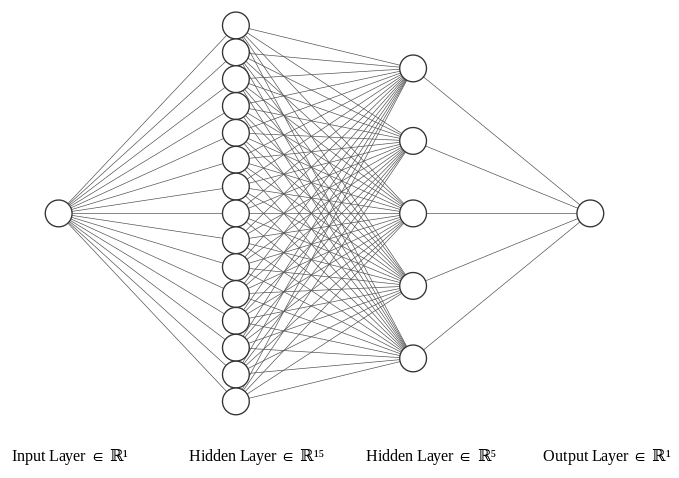
\includegraphics[width=0.7\textwidth]{figures/ann_1.png}
	\caption{Graphical representation of the ANN used to approximate the function $f(x) = x^3 + 2$.}
        \label{fig:ann_1}
\end{figure}

After the training is completed we can evaluate how good it is. To do
this we can compute the residuals or the square root of the sum of the
squared difference between the true value and the one predicted by the
NN. To have a numerical estimate of the agreement it has been computed also the
\emph{mean squared error} defined as:

\begin{equation}\textrm{MSE} = \cfrac{\sum_{i=1}^n{\big(\frac{x_{i}^{pred} - x_i^{truth}}{x_i^{truth}}\big)^2}}{n}\end{equation}
A \emph{perfect} prediction would lead to \(\textrm{MSE}=0\) so the
lower this number the better the agreement.

\begin{tcolorbox}[breakable, size=fbox, boxrule=1pt, pad at break*=1mm,colback=cellbackground, colframe=cellborder]
\begin{Verbatim}[commandchars=\\\{\}]
\PY{k+kn}{from} \PY{n+nn}{sklearn}\PY{n+nn}{.}\PY{n+nn}{metrics} \PY{k}{import} \PY{n}{mean\PYZus{}squared\PYZus{}error}
	
\PY{n}{trainer.fullPrediction()}
\PY{c+c1}{\PYZsh{} report model error computing the mean squared error}
\PY{n+nb}{print}\PY{p}{(}\PY{l+s+s1}{\PYZsq{}}\PY{l+s+s1}{MSE: }\PY{l+s+si}{\PYZpc{}.7f}\PY{l+s+s1}{\PYZsq{}} \PY{o}{\PYZpc{}} \PY{n}{mean\PYZus{}squared\PYZus{}error}\PY{p}{(}\PY{n}{trainer}\PY{o}{.}\PY{n}{y}\PY{p}{,} \PY{n}{trainer}\PY{o}{.}\PY{n}{predictions}\PY{p}{)}\PY{p}{)}

MSE: 0.0000062
\end{Verbatim}
\end{tcolorbox}

To get an idea of what it is going on in Fig.~\ref{fig:training_vs_epochs} are shown the
actual function we want to approximate and different predictions of our
NN obtained with four epoch numbers (5, 100, 800, 5000).

\begin{figure}[htb]
	\centering
	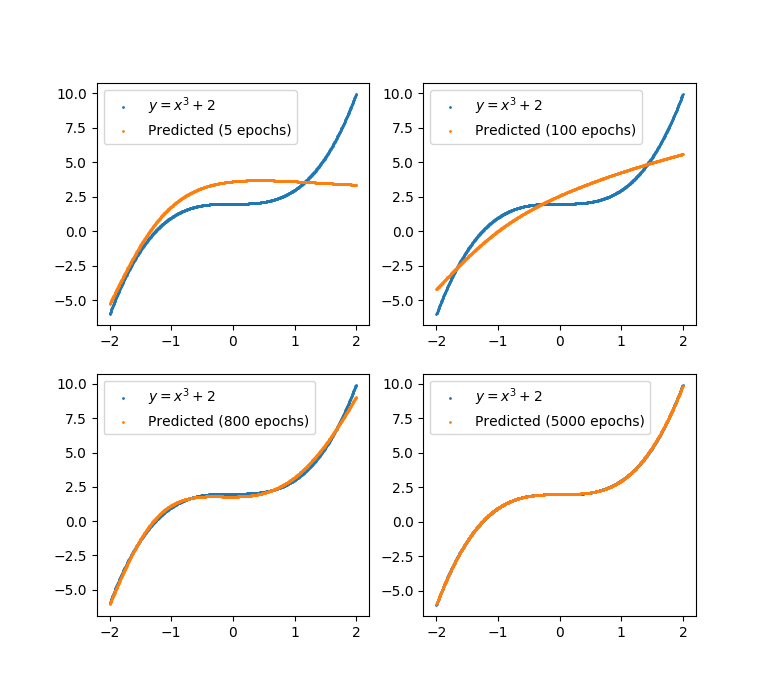
\includegraphics[width=0.7\textwidth]{figures/training_vs_epoch}
	\caption{Prediction of the target $f(x)$ using different number of epochs in the training (5, 100, 800 and 5000) respectively.}
	\label{fig:training_vs_epochs}
\end{figure}

It is clear how the agreement improves with higher number of epochs
which means that the NN has more opportunities to adapt the weights and
reduce the loss (or error or distance) to the target values. Even in the
case of 5000 epochs zooming in you could see discrepancies not visible
at the scale of the plot. Remember that increasing too much the number
of epochs may lead to overfitting. So in this case if we need more
accuracy we need to either increase the training sample or to change the
NN design.

To check if this is the case we can \emph{evaluate} our NN with both the
training ad the testing samples. If the losses are comparable the NN is
ok otherwise if the training losses are much smaller than the testing we
had overfitting.

\begin{tcolorbox}[breakable, size=fbox, boxrule=1pt, pad at break*=1mm,colback=cellbackground, colframe=cellborder]
\begin{Verbatim}[commandchars=\\\{\}]
\PY{n}{trainer}\PY{o}{.}\PY{n}{evaluate}\PY{p}{(}\PY{p}{)}

3200/3200 [==============================] - 0s 83us/step
Training: 6.1983578859781115e-06
800/800 [==============================] - 0s 52us/step
Test: 6.47684617433697e-06
\end{Verbatim}
\end{tcolorbox}

Since the two numbers are in good agreement we can be confident that our
NN didn't overfit.

\subsection{Black-Scholes call
options}\label{black-scholes-call-options}

The first financial application of a NN concerns the pricing of european
call options: essentially we will create a neural network capable of
approximate the famous Black-Scholes pricing formula

\begin{equation} P_\textrm{call} = F_\textrm{BS}(K, r, \sigma, \mathrm{ttm})\end{equation}

Like before we are going to generate the training sample this time made
of a grid of volatility-rate pairs \((\sigma, r)\) (for simplicity we
are going to set moneyness and time to maturity to 1). The target values
are the price of a call computed using the pricing function in the
\(\tt{finmarkets.py}\) library with the corresponding inputs.

\begin{tcolorbox}[breakable, size=fbox, boxrule=1pt, pad at break*=1mm,colback=cellbackground, colframe=cellborder]
\begin{Verbatim}[commandchars=\\\{\}]
\PY{k+kn}{from} \PY{n+nn}{finmarkets} \PY{k}{import} \PY{n}{call}
	
\PY{n}{data} \PY{o}{=} \PY{p}{[}\PY{p}{]}
\PY{n}{rates} \PY{o}{=} \PY{n}{np}\PY{o}{.}\PY{n}{arange}\PY{p}{(}\PY{l+m+mf}{0.01}\PY{p}{,} \PY{l+m+mf}{0.11}\PY{p}{,} \PY{l+m+mf}{0.001}\PY{p}{)}
\PY{n}{sigmas} \PY{o}{=} \PY{n}{np}\PY{o}{.}\PY{n}{arange}\PY{p}{(}\PY{l+m+mf}{0.1}\PY{p}{,} \PY{l+m+mf}{0.6}\PY{p}{,} \PY{l+m+mf}{0.005}\PY{p}{)}
	
\PY{k}{for} \PY{n}{r} \PY{o+ow}{in} \PY{n}{rates}\PY{p}{:}
    \PY{k}{for} \PY{n}{sigma} \PY{o+ow}{in} \PY{n}{sigmas}\PY{p}{:}
        \PY{n}{call\PYZus{}price} \PY{o}{=} \PY{n}{call}\PY{p}{(}\PY{l+m+mi}{1}\PY{p}{,} \PY{n}{r}\PY{p}{,} \PY{n}{sigma}\PY{p}{,} \PY{l+m+mi}{1}\PY{p}{)}
        \PY{n}{data}\PY{o}{.}\PY{n}{append}\PY{p}{(}\PY{p}{[}\PY{n}{r}\PY{p}{,} \PY{n}{sigma}\PY{p}{,} \PY{n}{call\PYZus{}price}\PY{p}{]}\PY{p}{)}
	
\PY{c+c1}{\PYZsh{} we transform the list to a numpy array just because }
\PY{c+c1}{\PYZsh{} an array it is more convenient to use later}
\PY{n}{data} \PY{o}{=} \PY{n}{np}\PY{o}{.}\PY{n}{array}\PY{p}{(}\PY{n}{data}\PY{p}{)}
\end{Verbatim}
\end{tcolorbox}

Since it takes some time to generate data samples, it is always
advisable to save them in a file since we may need to load it many times
during the NN development. This can be done with \(\tt{pandas}\).

\begin{tcolorbox}[breakable, size=fbox, boxrule=1pt, pad at break*=1mm,colback=cellbackground, colframe=cellborder]
\begin{Verbatim}[commandchars=\\\{\}]
\PY{k+kn}{import} \PY{n+nn}{pandas} \PY{k}{as} \PY{n+nn}{pd}
	
\PY{n}{df} \PY{o}{=} \PY{n}{pd}\PY{o}{.}\PY{n}{DataFrame}\PY{p}{(}\PY{p}{)}
\PY{n}{df}\PY{p}{[}\PY{l+s+s1}{\PYZsq{}}\PY{l+s+s1}{rate}\PY{l+s+s1}{\PYZsq{}}\PY{p}{]} \PY{o}{=} \PY{n}{data}\PY{p}{[}\PY{p}{:}\PY{p}{,} \PY{l+m+mi}{0}\PY{p}{]}
\PY{n}{df}\PY{p}{[}\PY{l+s+s1}{\PYZsq{}}\PY{l+s+s1}{vol}\PY{l+s+s1}{\PYZsq{}}\PY{p}{]} \PY{o}{=} \PY{n}{data}\PY{p}{[}\PY{p}{:}\PY{p}{,} \PY{l+m+mi}{1}\PY{p}{]}
\PY{n}{df}\PY{p}{[}\PY{l+s+s1}{\PYZsq{}}\PY{l+s+s1}{price}\PY{l+s+s1}{\PYZsq{}}\PY{p}{]} \PY{o}{=} \PY{n}{data}\PY{p}{[}\PY{p}{:}\PY{p}{,} \PY{l+m+mi}{2}\PY{p}{]}
	
\PY{n}{df}\PY{o}{.}\PY{n}{to\PYZus{}csv}\PY{p}{(}\PY{l+s+s2}{\PYZdq{}}\PY{l+s+s2}{bs\PYZus{}training\PYZus{}sample.csv}\PY{l+s+s2}{\PYZdq{}}\PY{p}{)}
\PY{n+nb}{print} \PY{p}{(}\PY{n}{df}\PY{o}{.}\PY{n}{describe}\PY{p}{(}\PY{p}{)}\PY{p}{)}

               rate           vol         price
count  10000.000000  10000.000000  10000.000000
mean       0.059500      0.347500      0.165274
std        0.028868      0.144338      0.055387
min        0.010000      0.100000      0.044852
25%        0.034750      0.223750      0.119389
50%        0.059500      0.347500      0.165476
75%        0.084250      0.471250      0.212097
max        0.109000      0.595000      0.277071
\end{Verbatim}
\end{tcolorbox}

Following the previous example we will use the \(\tt{FinNN}\) utility
class to develop the NN and also we will \emph{normalize} data to get
better results. \textbf{Beware that this time we have TWO input
  parameters (rate and volatilty)} and not just one. See Figure~\ref{fig:ann_2} for
a graphical representation of the used ANN.

\begin{tcolorbox}[breakable, size=fbox, boxrule=1pt, pad at break*=1mm,colback=cellbackground, colframe=cellborder]
\begin{Verbatim}[commandchars=\\\{\}]
\PY{n}{data} \PY{o}{=}  \PY{n}{pd}\PY{o}{.}\PY{n}{read\PYZus{}csv}\PY{p}{(}\PY{l+s+s2}{\PYZdq{}}\PY{l+s+s2}{bs\PYZus{}training\PYZus{}sample.csv}\PY{l+s+s2}{\PYZdq{}}\PY{p}{)}
	
\PY{n}{x} \PY{o}{=} \PY{n}{data}\PY{o}{.}\PY{n}{iloc}\PY{p}{[}\PY{p}{:}\PY{p}{,} \PY{l+m+mi}{1}\PY{p}{:}\PY{l+m+mi}{3}\PY{p}{]}\PY{o}{.}\PY{n}{values}
\PY{n}{y} \PY{o}{=} \PY{n}{data}\PY{o}{.}\PY{n}{iloc}\PY{p}{[}\PY{p}{:}\PY{p}{,} \PY{l+m+mi}{3}\PY{p}{]}\PY{o}{.}\PY{n}{values}

\PY{n}{trainer} \PY{o}{=} \PY{n}{FinNN}\PY{p}{(}\PY{l+s+s2}{\PYZdq{}}\PY{l+s+s2}{ANN}\PY{l+s+s2}{\PYZdq{}}\PY{p}{)}
\PY{n}{trainer}\PY{o}{.}\PY{n}{setData}\PY{p}{(}\PY{n}{x}\PY{p}{,} \PY{n}{y}\PY{p}{,} \PY{n}{test\PYZus{}size}\PY{o}{=}\PY{l+m+mf}{0.20}\PY{p}{)}
\PY{n}{trainer}\PY{o}{.}\PY{n}{normalize}\PY{p}{(}\PY{p}{)}
	
\PY{c+c1}{\PYZsh{} define the NN architecture}
\PY{n}{trainer}\PY{o}{.}\PY{n}{addInputLayer}\PY{p}{(}\PY{n}{inputs}\PY{o}{=}\PY{l+m+mi}{2}\PY{p}{,} \PY{n}{neurons}\PY{o}{=}\PY{l+m+mi}{20}\PY{p}{,} \PY{n}{activation}\PY{o}{=}\PY{l+s+s1}{\PYZsq{}}\PY{l+s+s1}{relu}\PY{l+s+s1}{\PYZsq{}}\PY{p}{)}
\PY{n}{trainer}\PY{o}{.}\PY{n}{addHiddenLayer}\PY{p}{(}\PY{n}{neurons}\PY{o}{=}\PY{l+m+mi}{8}\PY{p}{,} \PY{n}{activation}\PY{o}{=}\PY{l+s+s1}{\PYZsq{}}\PY{l+s+s1}{relu}\PY{l+s+s1}{\PYZsq{}}\PY{p}{)}
\PY{n}{trainer}\PY{o}{.}\PY{n}{addOutputLayer}\PY{p}{(}\PY{n}{outputs}\PY{o}{=}\PY{l+m+mi}{1}\PY{p}{)}
\PY{n}{trainer}\PY{o}{.}\PY{n}{compileModel}\PY{p}{(}\PY{n}{loss}\PY{o}{=}\PY{l+s+s1}{\PYZsq{}}\PY{l+s+s1}{mse}\PY{l+s+s1}{\PYZsq{}}\PY{p}{,} \PY{n}{opt}\PY{o}{=}\PY{l+s+s1}{\PYZsq{}}\PY{l+s+s1}{adam}\PY{l+s+s1}{\PYZsq{}}\PY{p}{)}
	
\PY{n}{trainer}\PY{o}{.}\PY{n}{fit}\PY{p}{(}\PY{n}{epochs}\PY{o}{=}\PY{l+m+mi}{3000}\PY{p}{,} \PY{n}{batch\PYZus{}size}\PY{o}{=}\PY{l+m+mi}{500}\PY{p}{,} \PY{n}{verbose}\PY{o}{=}\PY{l+m+mi}{1}\PY{p}{)}

Epoch 1/3000
8000/8000 [==============================] - 0s 16us/step - loss: 0.3216
Epoch 2/3000
8000/8000 [==============================] - 0s 4us/step - loss: 0.2620
...
Epoch 2999/3000
8000/8000 [==============================] - 0s 4us/step - loss: 3.7983e-07
Epoch 3000/3000
8000/8000 [==============================] - 0s 3us/step - loss: 3.6476e-07

\PY{n}{trainer}\PY{o}{.}\PY{n}{evaluate}\PY{p}{(}\PY{p}{)}
	
\PY{c+c1}{\PYZsh{} when the training takes some time it is useful}
\PY{c+c1}{\PYZsh{} to save the model weights in a file to use it later on}
\PY{n}{trainer}\PY{o}{.}\PY{n}{saveModel}\PY{p}{(}\PY{l+s+s1}{\PYZsq{}}\PY{l+s+s1}{black\PYZus{}scholes}\PY{l+s+s1}{\PYZsq{}}\PY{p}{)}

8000/8000 [==============================] - 0s 52us/step
Training: 5.567638540924235e-07
2000/2000 [==============================] - 0s 44us/step
Test: 5.582978365055169e-07
\end{Verbatim}
\end{tcolorbox}

\begin{figure}[htb]
	\centering
	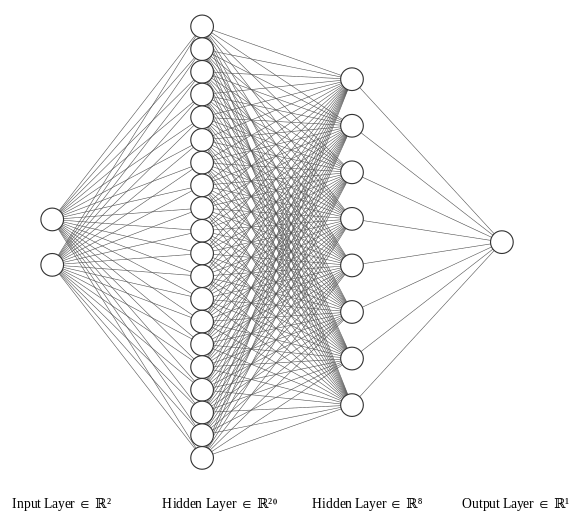
\includegraphics[width=0.7\textwidth]{figures/ann_2.png}
	\caption{Graphical representation of the ANN used to approximate the Black and Scholes oprion price function.}
        \label{fig:ann_2}
\end{figure}

As you can see the training and test samples give roughly the same MSE
value so we are reasonably sure that there hasn't been
\emph{overfitting}.
After the training is completed again we can
evaluate graphically how good it is, see Fig.~\ref{fig:vol_rate}. 

\begin{figure}[htb]
	\centering
	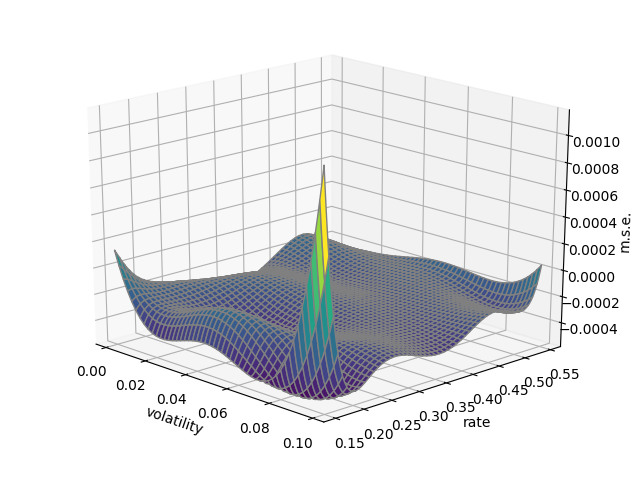
\includegraphics[width=0.7\textwidth]{figures/vol_rate}
	\caption{Mean squared error as a function of volatility and rate for our Black-Scholes function prediction.}
	\label{fig:vol_rate}
\end{figure}

In general to judge if the level of accuracy we have reached is enough
you have to

\begin{itemize}
	\tightlist
	\item
	if you are using the metric MSE you need to make the
	\(\sqrt{\mathrm{MSE}}\) to get the \emph{real} error
	\item
	apply this error to a typical output and check if the accuracy is
	enough.
\end{itemize}

In this example we know that our prices go from 0.04 to 0.28 and the
final accuracy is 0.0007. So in the
worst case we are able to price our call as \(0.04 \pm 0.0007\), which
is not bad for our study but may not be ideal for deciding if we would
like to invest in this call or not.

We can compare the prediction in a practical case; let's say we
want to know the price of a call (with moneyness 1 and time to maturity
1 year) when the risk-free rate is 0.015 and the volatility 0.234:

\begin{tcolorbox}[breakable, size=fbox, boxrule=1pt, pad at break*=1mm,colback=cellbackground, colframe=cellborder]
\begin{Verbatim}[commandchars=\\\{\}]
\PY{k+kn}{import} \PY{n+nn}{numpy} \PY{k}{as} \PY{n+nn}{np}
\PY{k+kn}{from} \PY{n+nn}{finmarkets} \PY{k}{import} \PY{n}{call}
	
\PY{c+c1}{\PYZsh{} here we load the trained model}
\PY{n}{trainer}\PY{o}{.}\PY{n}{loadModel}\PY{p}{(}\PY{l+s+s1}{\PYZsq{}}\PY{l+s+s1}{black\PYZus{}scholes}\PY{l+s+s1}{\PYZsq{}}\PY{p}{)}
	
\PY{c+c1}{\PYZsh{} this is our input vector}
\PY{n}{rv} \PY{o}{=} \PY{n}{np}\PY{o}{.}\PY{n}{array}\PY{p}{(}\PY{p}{[}\PY{p}{[}\PY{l+m+mf}{0.015}\PY{p}{,} \PY{l+m+mf}{0.234}\PY{p}{]}\PY{p}{]}\PY{p}{)}
\PY{c+c1}{\PYZsh{} here we compare the predection with the BS call price}
\PY{n+nb}{print} \PY{p}{(}\PY{l+s+s1}{\PYZsq{}}\PY{l+s+si}{\PYZob{}\PYZcb{}}\PY{l+s+s1}{ =\PYZgt{} }\PY{l+s+si}{\PYZob{}:.4f\PYZcb{}}\PY{l+s+s1}{ (expected }\PY{l+s+si}{\PYZob{}:.4f\PYZcb{}}\PY{l+s+s1}{)}\PY{l+s+s1}{\PYZsq{}}\PY{o}{.}\PY{n}{format}\PY{p}{(}\PY{n}{rv}\PY{o}{.}\PY{n}{tolist}\PY{p}{(}\PY{p}{)}\PY{p}{,} 
                                               \PY{n}{trainer}\PY{o}{.}\PY{n}{predict}\PY{p}{(}\PY{n}{rv}\PY{p}{)}\PY{p}{[}\PY{l+m+mi}{0}\PY{p}{]}\PY{p}{[}\PY{l+m+mi}{0}\PY{p}{]}\PY{p}{,} 
                                               \PY{n}{call}\PY{p}{(}\PY{l+m+mi}{1}\PY{p}{,} \PY{n}{rv}\PY{p}{[}\PY{l+m+mi}{0}\PY{p}{]}\PY{p}{[}\PY{l+m+mi}{0}\PY{p}{]}\PY{p}{,} \PY{n}{rv}\PY{p}{[}\PY{l+m+mi}{0}\PY{p}{]}\PY{p}{[}\PY{l+m+mi}{1}\PY{p}{]}\PY{p}{,} \PY{l+m+mi}{1}\PY{p}{)}\PY{p}{)}\PY{p}{)}

[[0.015, 0.234]] => 0.1001 (expected 0.1001)
\end{Verbatim}
\end{tcolorbox}

It is very import to remeber that a \textbf{NN cannot estrapolate}.
Indeed if you try to predict the price of a call from rate and
volatility outside the training \emph{phase space} (with values that
aren't in the intervals used in the training), say \(r = 0.22\) and
\(\sigma = 0.01\)\ldots{}

\begin{tcolorbox}[breakable, size=fbox, boxrule=1pt, pad at break*=1mm,colback=cellbackground, colframe=cellborder]
\begin{Verbatim}[commandchars=\\\{\}]
\PY{c+c1}{\PYZsh{} this is our input vector}
\PY{n}{rv} \PY{o}{=} \PY{n}{np}\PY{o}{.}\PY{n}{array}\PY{p}{(}\PY{p}{[}\PY{p}{[}\PY{l+m+mf}{0.22}\PY{p}{,} \PY{l+m+mf}{0.01}\PY{p}{]}\PY{p}{]}\PY{p}{)}
	
\PY{c+c1}{\PYZsh{} here we compare the predection with the BS call price}
\PY{n+nb}{print} \PY{p}{(}\PY{l+s+s1}{\PYZsq{}}\PY{l+s+si}{\PYZob{}\PYZcb{}}\PY{l+s+s1}{ =\PYZgt{} }\PY{l+s+si}{\PYZob{}:.4f\PYZcb{}}\PY{l+s+s1}{ (expected }\PY{l+s+si}{\PYZob{}:.4f\PYZcb{}}\PY{l+s+s1}{)}\PY{l+s+s1}{\PYZsq{}}\PY{o}{.}\PY{n}{format}\PY{p}{(}\PY{n}{rv}\PY{o}{.}\PY{n}{tolist}\PY{p}{(}\PY{p}{)}\PY{p}{,} 
                                               \PY{n}{trainer}\PY{o}{.}\PY{n}{predict}\PY{p}{(}\PY{n}{rv}\PY{p}{)}\PY{p}{[}\PY{l+m+mi}{0}\PY{p}{]}\PY{p}{[}\PY{l+m+mi}{0}\PY{p}{]}\PY{p}{,} 
                                               \PY{n}{call}\PY{p}{(}\PY{l+m+mi}{1}\PY{p}{,} \PY{n}{rv}\PY{p}{[}\PY{l+m+mi}{0}\PY{p}{]}\PY{p}{[}\PY{l+m+mi}{0}\PY{p}{]}\PY{p}{,} \PY{n}{rv}\PY{p}{[}\PY{l+m+mi}{0}\PY{p}{]}\PY{p}{[}\PY{l+m+mi}{1}\PY{p}{]}\PY{p}{,} \PY{l+m+mi}{1}\PY{p}{)}\PY{p}{)}\PY{p}{)}

[[0.22, 0.01]] => 0.1628 (expected 0.1975)
\end{Verbatim}
\end{tcolorbox}

\subsection{Model Calibration}\label{model-calibration}

The function approximation capabilities of a neural network can serve
other scopes rather than predicting the function values. A very useful
application is indeed \emph{model calibration} which consists of
deriving parameters of a model directly from market values. This is
especially convenient to estimate parameters (e.g. volatility) which are
otherwise complicated to compute.

Assume we need to estimate the \emph{implied volatility} of a stock price
in real time. If in the market are available call options with our stock
as underlying we can exploit again the Black and Scholes formula. The
idea is in fact to train a NN where the input is a list of price,
moneyness, rate and time to maturity
\((P_\textrm{call}, K, r, \mathrm{ttm})\) and the target output is the
volatility. In our examples of function approximation we have never made any assumption on the functional form but we have just relied on the capability of NN to learn from the training dataset. So now we can reuse the same data used before to solve

\begin{equation} \sigma = F^{-1}_\textrm{BS}(P_\textrm{call}, K, r, \mathrm{ttm})\end{equation}

We can than calibrate our model by predicting the stock volatility with
the trained NN using as input the market price of the option and its
characteristics.

\subsubsection{Historical vs.~Implied
		Volatility}\label{historical-vs.-implied-volatility}

Historical volatility is the realized volatility of the underlying asset over a previous time period. It is determined by measuring the standard deviation of the underlying asset from the mean during that time period.

In contrast to historical volatility, which looks at actual stock prices in the past, implied volatility looks toward the future. Implied volatility is often interpreted as the market's expectation for the future volatility of a stock and can be derived from the price of an option (e.g. from the Black and Scholes formula).
Specifically, it is the expected future volatility of the stock that is implied by the price of the stock's options.

The implied volatility of an asset can also be compared with what it was in the past. If a stock has an implied volatility of 40\% compared with a 20\% implied volatility, say, a month ago, the market now considers the stock to be more volatile particularly going forward.

Volatility shifts as markets go through different regimes. Thus, historical volatility may not be an accurate measure of future volatility. Implied volatility
takes into account all of the information used by market participants to 
determine prices in the options market, instead of just past prices.

In general, if implied volatility is higher than historical volatility it gives some indication that option prices may be high. If implied volatility is below historical volatility, this may mean option prices are discounted and may be “cheap.”

To reuse the training sample created before (again we
are going to set \(\mathrm{ttm}=1\) and \(K=1\)) now \(\tt{x}\) we need to set the input as pairs of rate and price and \(\tt{y}\) will be the target volatility.

\begin{tcolorbox}[breakable, size=fbox, boxrule=1pt, pad at break*=1mm,colback=cellbackground, colframe=cellborder]
\begin{Verbatim}[commandchars=\\\{\}]
\PY{k+kn}{import} \PY{n+nn}{pandas} \PY{k}{as} \PY{n+nn}{pd}
\PY{k+kn}{from} \PY{n+nn}{finnn} \PY{k}{import} \PY{n}{FinNN}
	
\PY{n}{data} \PY{o}{=}  \PY{n}{pd}\PY{o}{.}\PY{n}{read\PYZus{}csv}\PY{p}{(}\PY{l+s+s2}{\PYZdq{}}\PY{l+s+s2}{bs\PYZus{}training\PYZus{}sample.csv}\PY{l+s+s2}{\PYZdq{}}\PY{p}{)}
\PY{n}{df} \PY{o}{=} \PY{n}{pd}\PY{o}{.}\PY{n}{concat([data.iloc[:, 1:2], data.iloc[:, 3:4]], 1)}\PY{p}{)}
\PY{n}{x} \PY{o}{=} \PY{n}{df}\PY{o}{.}\PY{n}{values}
\PY{n}{y} \PY{o}{=} \PY{n}{data}\PY{o}{.}\PY{n}{iloc}\PY{p}{[}\PY{p}{:}\PY{p}{,} \PY{l+m+mi}{1}\PY{p}{]}\PY{o}{.}\PY{n}{values}

\PY{n}{trainer} \PY{o}{=} \PY{n}{FinNN}\PY{p}{(}\PY{l+s+s2}{\PYZdq{}}\PY{l+s+s2}{ANN}\PY{l+s+s2}{\PYZdq{}}\PY{p}{)}
\PY{n}{trainer}\PY{o}{.}\PY{n}{setData}\PY{p}{(}\PY{n}{x}\PY{p}{,} \PY{n}{y}\PY{p}{,} \PY{n}{test\PYZus{}size}\PY{o}{=}\PY{l+m+mf}{0.20}\PY{p}{)}
\PY{n}{trainer}\PY{o}{.}\PY{n}{normalize}\PY{p}{(}\PY{p}{)}
	
\PY{n}{trainer}\PY{o}{.}\PY{n}{addInputLayer}\PY{p}{(}\PY{n}{inputs}\PY{o}{=}\PY{l+m+mi}{2}\PY{p}{,} \PY{n}{neurons}\PY{o}{=}\PY{l+m+mi}{20}\PY{p}{,} \PY{n}{activation}\PY{o}{=}\PY{l+s+s1}{\PYZsq{}}\PY{l+s+s1}{relu}\PY{l+s+s1}{\PYZsq{}}\PY{p}{)}
\PY{n}{trainer}\PY{o}{.}\PY{n}{addHiddenLayer}\PY{p}{(}\PY{n}{neurons}\PY{o}{=}\PY{l+m+mi}{8}\PY{p}{,} \PY{n}{activation}\PY{o}{=}\PY{l+s+s1}{\PYZsq{}}\PY{l+s+s1}{relu}\PY{l+s+s1}{\PYZsq{}}\PY{p}{)}
\PY{n}{trainer}\PY{o}{.}\PY{n}{addOutputLayer}\PY{p}{(}\PY{n}{outputs}\PY{o}{=}\PY{l+m+mi}{1}\PY{p}{)}

\PY{n}{trainer}\PY{o}{.}\PY{n}{compileModel}\PY{p}{(}\PY{n}{loss}\PY{o}{=}\PY{l+s+s1}{\PYZsq{}}\PY{l+s+s1}{mse}\PY{l+s+s1}{\PYZsq{}}\PY{p}{,} \PY{n}{opt}\PY{o}{=}\PY{l+s+s1}{\PYZsq{}}\PY{l+s+s1}{adam}\PY{l+s+s1}{\PYZsq{}}\PY{p}{)}
\PY{n}{trainer}\PY{o}{.}\PY{n}{fit}\PY{p}{(}\PY{n}{epochs}\PY{o}{=}\PY{l+m+mi}{2000}\PY{p}{,}  \PY{n}{verbose}\PY{o}{=}\PY{l+m+mi}{1}\PY{p}{)}
	
\PY{n}{trainer}\PY{o}{.}\PY{n}{evaluate}\PY{p}{(}\PY{p}{)}
\PY{n}{trainer}\PY{o}{.}\PY{n}{saveModel}\PY{p}{(}\PY{l+s+s2}{\PYZdq{}}\PY{l+s+s2}{calibration}\PY{l+s+s2}{\PYZdq{}}\PY{p}{)}

Epoch 1/2000
8000/8000 [==============================] - 0s 14us/step - loss: 0.1339
Epoch 2/2000
8000/8000 [==============================] - 0s 4us/step - loss: 0.1052
...
Epoch 1999/2000
8000/8000 [==============================] - 0s 10us/step - loss: 1.9519e-06
Epoch 2000/2000
8000/8000 [==============================] - 0s 10us/step - loss: 1.9708e-06

8000/8000 [==============================] - 0s 61us/step
Training: 2.0318084630162047e-06
2000/2000 [==============================] - 0s 48us/step
Test: 1.8580968553578714e-06
\end{Verbatim}
\end{tcolorbox}

Provided our training includes the correct range of market prices of our
call we can quickly and easily estimate the implied volatility. For
example if the risk-free rate is 2\% and the current price is 0.15
(remember that we are using the BS formula in terms of moneyness)

\begin{tcolorbox}[breakable, size=fbox, boxrule=1pt, pad at break*=1mm,colback=cellbackground, colframe=cellborder]
\begin{Verbatim}[commandchars=\\\{\}]
\PY{n}{trainer}\PY{o}{.}\PY{n}{loadModel}\PY{p}{(}\PY{l+s+s1}{\PYZsq{}}\PY{l+s+s1}{calibration}\PY{l+s+s1}{\PYZsq{}}\PY{p}{)}
\PY{n}{rv} \PY{o}{=} \PY{n}{np}\PY{o}{.}\PY{n}{array}\PY{p}{(}\PY{p}{[}\PY{p}{[}\PY{l+m+mf}{0.02}\PY{p}{,} \PY{l+m+mf}{0.15}\PY{p}{]}\PY{p}{]}\PY{p}{)}
	
\PY{n+nb}{print} \PY{p}{(}\PY{l+s+s1}{\PYZsq{}}\PY{l+s+si}{\PYZob{}\PYZcb{}}\PY{l+s+s1}{ =\PYZgt{} }\PY{l+s+si}{\PYZob{}:.4f\PYZcb{}}\PY{l+s+s1}{ (expected call price }\PY{l+s+si}{\PYZob{}:.4f\PYZcb{}}\PY{l+s+s1}{)}\PY{l+s+s1}{\PYZsq{}}\PY{o}{.}\PY{n}{format}\PY{p}{(}\PY{n}{rv}\PY{o}{.}\PY{n}{tolist}\PY{p}{(}\PY{p}{)}\PY{p}{,} 
                                               \PY{n}{trainer}\PY{o}{.}\PY{n}{predict}\PY{p}{(}\PY{n}{rv}\PY{p}{)}\PY{p}{[}\PY{l+m+mi}{0}\PY{p}{]}\PY{p}{[}\PY{l+m+mi}{0}\PY{p}{]}\PY{p}{,} 
                                               \PY{n}{call}\PY{p}{(}\PY{l+m+mi}{1}\PY{p}{,} \PY{l+m+mf}{0.02}\PY{p}{,} 
                                                    \PY{n}{trainer}\PY{o}{.}\PY{n}{predict}\PY{p}{(}\PY{n}{rv}\PY{p}{)}\PY{p}{[}\PY{l+m+mi}{0}\PY{p}{]}\PY{p}{[}\PY{l+m+mi}{0}\PY{p}{]}\PY{p}{,} \PY{l+m+mi}{1}\PY{p}{)}\PY{p}{)}\PY{p}{)}

[[0.02, 0.15]] => 0.3565 (expected call price 0.1502)
\end{Verbatim}
\end{tcolorbox}

\section{Neural net to recognize handwritten
		digits}\label{neural-net-to-recognize-handwritten-digits}

We don't usually appreciate how tough a problem our visual system solve,
maybe it is enough to consider that it involves 5 visual cortices
containing 140 million neurons each. Anyway the difficulties of visual
pattern recognition become apparent if you attempt to write a computer
program to recognize digits like those in Fig.~\ref{fig:mnist}

\begin{figure}[htb]
	\centering
	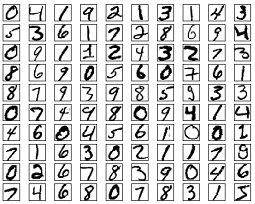
\includegraphics[width=0.5\textwidth]{figures/mnist_100_digits}
	\caption{MNIST sample of handwritten digits.}
	\label{fig:mnist}
\end{figure}

Simple intuition about how we recognize shapes (e.g.~a 9 has a loop at
the top, and a vertical stroke in the bottom right) turns out to be not
so simple to express algorithmically. When you try to make such rules
precise, you quickly get lost in a morass of exceptions and caveats and
special cases so that it seems hopeless.

Neural networks approach the problem in a different way. The idea is to
take a large number of handwritten digits and then develop a system
which can learn from those.

By increasing the number of training examples, the network can learn
more and more about handwriting, and so improve its accuracy. So while
it has been shown just 100 training digits above, we could certainly
build a better handwriting recognizer by using thousands or even
millions or billions of training examples (\textbf{as we have seen above
	neural nets are not capable of extrapolating results, hence it won't
	recongnize a digit written in some strange way not included in the
	training sample !!!}).

Let's first try to implement a NN that is capable of recognizing
handwritten digits. In this example we will use tha sample provided with
the \(\tt{mnist}\) module.

Our program will be based on a slightly different kind of neural network
than before, one type specifically designed for image/pattern
recognition, the Convolutional Neural Network (CNN). We won't go into
the details of its implementation since it is outside the scope of these
lectures but it works essentially by applying on top of an image a
series of filters (\emph{convolutional layers}) that works as edge
detectors. With them it classifies the images according to their
relevant features.

Convolutional layers prove very effective, and stacking them allows to
learn low-level features (e.g. lines) and high-order (more abstract)
features, like shapes or specific objects, see FIg.~\ref{fig:conv_filters}.

\begin{figure}[htb]
	\centering
	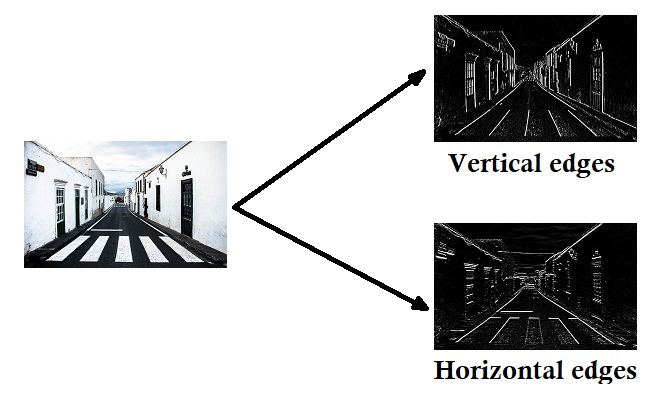
\includegraphics[width=1.\textwidth]{figures/edges.jpg}
	\caption{Edge detected by different layers of a convolutional neural network.}
        \label{fig:conv_fitlers}
\end{figure}

Another important difference with respect to the previous examples is
that in this case we are going to solve a classification problem
(contrary to before when we were trying to regress a sample). Indeed our
NN output won't be a single number but rather a list containing the
probabilties that an image belonged to each class.

\begin{tcolorbox}[breakable, size=fbox, boxrule=1pt, pad at break*=1mm,colback=cellbackground, colframe=cellborder]
\begin{Verbatim}[commandchars=\\\{\}]
\PY{k+kn}{import} \PY{n+nn}{numpy} \PY{k}{as} \PY{n+nn}{np}\PY{o}{,} \PY{n+nn}{mnist}
\PY{k+kn}{from} \PY{n+nn}{finnn} \PY{k}{import} \PY{n}{FinNN}
	
\PY{c+c1}{\PYZsh{} the actual images}
\PY{n}{train\PYZus{}images} \PY{o}{=} \PY{n}{mnist}\PY{o}{.}\PY{n}{train\PYZus{}images}\PY{p}{(}\PY{p}{)} 
\PY{c+c1}{\PYZsh{} the target (it is a 0, 1, 2...)}
\PY{n}{train\PYZus{}labels} \PY{o}{=} \PY{n}{mnist}\PY{o}{.}\PY{n}{train\PYZus{}labels}\PY{p}{(}\PY{p}{)} 
	
\PY{c+c1}{\PYZsh{} no test\PYZus{}size option means not split the sample}
\PY{c+c1}{\PYZsh{} in training and testing sets}
\PY{c+c1}{\PYZsh{} (MNIST has already dont it for us)}
\PY{n}{trainer} \PY{o}{=} \PY{n}{FinNN}\PY{p}{(}\PY{l+s+s2}{\PYZdq{}}\PY{l+s+s2}{CNN2D}\PY{l+s+s2}{\PYZdq{}}\PY{p}{)}
\PY{n}{trainer}\PY{o}{.}\PY{n}{setData}\PY{p}{(}\PY{n}{train\PYZus{}images}\PY{p}{,} \PY{n}{train\PYZus{}labels}\PY{p}{)}
\end{Verbatim}
\end{tcolorbox}

Next we define the CNN architecture, see Fig.~\ref{fig:cnn2d}.

\begin{tcolorbox}[breakable, size=fbox, boxrule=1pt, pad at break*=1mm,colback=cellbackground, colframe=cellborder]
\begin{Verbatim}[commandchars=\\\{\}]
\PY{c+c1}{\PYZsh{} define our convolutional NN}
\PY{c+c1}{\PYZsh{} we decide to apply 8 filters to the images }
\PY{c+c1}{\PYZsh{} each with 3x3 pixels size}
\PY{c+c1}{\PYZsh{} the input images have 28x28 pixels size instead}
\PY{n}{trainer}\PY{o}{.}\PY{n}{addConv2DLayer}\PY{p}{(}\PY{n}{filters}\PY{o}{=}\PY{l+m+mi}{8}\PY{p}{,} \PY{n}{filter\PYZus{}size}\PY{o}{=}\PY{l+m+mi}{3}\PY{p}{,} \PY{n}{input\PYZus{}shape}\PY{o}{=}\PY{p}{(}\PY{l+m+mi}{28}\PY{p}{,} \PY{l+m+mi}{28}\PY{p}{,} \PY{l+m+mi}{1}\PY{p}{)}\PY{p}{)}
\PY{n}{trainer}\PY{o}{.}\PY{n}{addMaxPooling2D}\PY{p}{(}\PY{l+m+mi}{2}\PY{p}{)}
\PY{n}{trainer}\PY{o}{.}\PY{n}{addFlatten}\PY{p}{(}\PY{p}{)}
\PY{n}{trainer}\PY{o}{.}\PY{n}{addCNNOutputLayer}\PY{p}{(}\PY{n}{outputs}\PY{o}{=}\PY{l+m+mi}{10}\PY{p}{)}
	
\PY{n}{trainer}\PY{o}{.}\PY{n}{compileModel}\PY{p}{(}\PY{n}{loss}\PY{o}{=}\PY{l+s+s1}{\PYZsq{}}\PY{l+s+s1}{categorical\PYZus{}crossentropy}\PY{l+s+s1}{\PYZsq{}}\PY{p}{,} \PY{n}{opt}\PY{o}{=}\PY{l+s+s1}{\PYZsq{}}\PY{l+s+s1}{adam}\PY{l+s+s1}{\PYZsq{}}\PY{p}{)}
	
\PY{c+c1}{\PYZsh{} no batch\PYZus{}size means batch\PYZus{}size=len(images)}
\PY{n}{trainer}\PY{o}{.}\PY{n}{fit}\PY{p}{(}\PY{n}{epochs}\PY{o}{=}\PY{l+m+mi}{5}\PY{p}{,} \PY{n}{verbose}\PY{o}{=}\PY{l+m+mi}{1}\PY{p}{)}
\PY{n}{trainer}\PY{o}{.}\PY{n}{saveModel}\PY{p}{(}\PY{l+s+s1}{\PYZsq{}}\PY{l+s+s1}{digit\PYZus{}training}\PY{l+s+s1}{\PYZsq{}}\PY{p}{)}

Epoch 1/5
59999/59999 [==============================] - 13s 210us/step - loss: 2.1711
Epoch 2/5
59999/59999 [==============================] - 12s 201us/step - loss: 0.3964
Epoch 3/5
59999/59999 [==============================] - 12s 199us/step - loss: 0.2655
Epoch 4/5
59999/59999 [==============================] - 12s 198us/step - loss: 0.2244
Epoch 5/5
59999/59999 [==============================] - 12s 196us/step - loss: 0.1910
\end{Verbatim}
\end{tcolorbox}

\begin{figure}[htb]
	\centering
	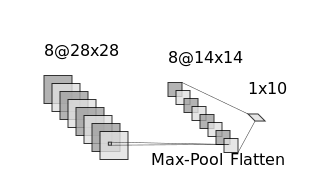
\includegraphics[width=0.7\textwidth]{figures/cnn_2d.png}
	\caption{Graphical representation of the CNN developed to recognize handwritten digits.}
        \label{fig:cnn2d}
\end{figure}

\begin{tcolorbox}[breakable, size=fbox, boxrule=1pt, pad at break*=1mm, colframe=cellborder, colback=cream]
\subsubsection{For the Most Curious}\label{for-the-most-curious}

If you look closely to the \(\tt{finnn.py}\) module you will notice that
I have cheated when describing the CNN architecture. In particular I
have not mentioned the \(\tt{MaxPooling2}\) layer, so let's clarify its
feature.

Convolutional layers in a convolutional neural network systematically
apply learned filters to input images in order to create feature maps
that summarize the presence of those features in the input.

A limitation of the feature map output of convolutional layers is that
they record the precise position of features in the input. This means
that small movements in the position of the feature in the input image
will result in a different feature map. This can happen with
re-cropping, rotation, shifting, and other minor changes to the input
image.

Imagine a program that look for car plates in pictures taken by a speed
radar, cars won't be in the same position in the frame so there may be
differences in the classification of similar (but not equal) pictures.

A common approach to address this problem from signal processing is
called \emph{down sampling}. This is where a lower resolution version of
an input signal (e.g.~the picture) is created that still contains the
large or important structural elements, without the fine detail that may
not be as useful to the task.

Down sampling can be achieved using a pooling layer.

Pooling involves selecting a pooling operation, much like a filter to be
applied to feature maps. The size of the pooling operation or filter is
smaller than the size of the feature map; specifically, it is almost
always 2×2 pixels. This means that the pooling layer will always reduce
the size of each feature map by a factor of 2, e.g.~each dimension is
halved. For example, a pooling layer applied to a feature map of 6×6 (36
pixels) will result in an output pooled feature map of 3×3 (9 pixels).

The most common pooling operation are: * Average Pooling: calculate the
average value for each patch on the feature map; * Maximum Pooling (or
Max Pooling): calculate the maximum value for each patch of the feature
map.
\end{tcolorbox}

Now let's try to see how well our NN predicts \(\tt{mnist}\) testing
digits.

\begin{tcolorbox}[breakable, size=fbox, boxrule=1pt, pad at break*=1mm,colback=cellbackground, colframe=cellborder]
\begin{Verbatim}[commandchars=\\\{\}]
\PY{n}{trainer}\PY{o}{.}\PY{n}{loadModel}\PY{p}{(}\PY{l+s+s1}{\PYZsq{}}\PY{l+s+s1}{digit\PYZus{}training}\PY{l+s+s1}{\PYZsq{}}\PY{p}{)}
	
\PY{c+c1}{\PYZsh{} testing with mnist test sample}
\PY{n}{test\PYZus{}images} \PY{o}{=} \PY{n}{mnist}\PY{o}{.}\PY{n}{test\PYZus{}images}\PY{p}{(}\PY{p}{)}
\PY{n}{test\PYZus{}labels} \PY{o}{=} \PY{n}{mnist}\PY{o}{.}\PY{n}{test\PYZus{}labels}\PY{p}{(}\PY{p}{)}
	
\PY{n}{trainer}\PY{o}{.}\PY{n}{setTestData}\PY{p}{(}\PY{n}{test\PYZus{}images}\PY{p}{,} \PY{n}{test\PYZus{}labels}\PY{p}{)}
\PY{n}{predictions} \PY{o}{=} \PY{n}{trainer}\PY{o}{.}\PY{n}{predict}\PY{p}{(}\PY{n}{trainer}\PY{o}{.}\PY{n}{x\PYZus{}test}\PY{p}{[}\PY{p}{:}\PY{l+m+mi}{10}\PY{p}{]}\PY{p}{)}
\PY{n+nb}{print} \PY{p}{(}\PY{l+s+s2}{\PYZdq{}}\PY{l+s+s2}{Tesing on MNIST digits...}\PY{l+s+s2}{\PYZdq{}}\PY{p}{)}
\PY{n+nb}{print}\PY{p}{(}\PY{l+s+s2}{\PYZdq{}}\PY{l+s+s2}{Predicted: }\PY{l+s+s2}{\PYZdq{}}\PY{p}{,} \PY{n}{np}\PY{o}{.}\PY{n}{argmax}\PY{p}{(}\PY{n}{predictions}\PY{p}{,} \PY{n}{axis}\PY{o}{=}\PY{l+m+mi}{1}\PY{p}{)}\PY{p}{)} 
\PY{n+nb}{print}\PY{p}{(}\PY{l+s+s2}{\PYZdq{}}\PY{l+s+s2}{Truth:}\PY{l+s+s2}{\PYZdq{}}\PY{p}{,} \PY{n}{test\PYZus{}labels}\PY{p}{[}\PY{p}{:}\PY{l+m+mi}{10}\PY{p}{]}\PY{p}{)}
	
\PY{c+c1}{\PYZsh{} this line returns the highest probability of the vector}
\PY{n+nb}{print}\PY{p}{(}\PY{l+s+s2}{\PYZdq{}}\PY{l+s+s2}{highest prob.:}\PY{l+s+s2}{\PYZdq{}}\PY{p}{,} \PY{p}{[}\PY{l+s+s2}{\PYZdq{}}\PY{l+s+si}{\PYZob{}:.6f\PYZcb{}}\PY{l+s+s2}{\PYZdq{}}\PY{o}{.}\PY{n}{format}\PY{p}{(}\PY{n}{p}\PY{p}{[}\PY{n}{np}\PY{o}{.}\PY{n}{argmax}\PY{p}{(}\PY{n}{p}\PY{p}{)}\PY{p}{]}\PY{p}{)} \PY{k}{for} \PY{n}{p} \PY{o+ow}{in} \PY{n}{predictions}\PY{p}{]}\PY{p}{)}

Tesing on MNIST digits{\ldots}
Predicted:  [7 2 1 0 4 1 4 4 5 9]
Truth: [7 2 1 0 4 1 4 9 5 9]
highest prob.: ['0.999900', '1.000000', '0.999977', '1.000000', '0.999993',
'0.999596', '0.970003', '0.900420', '0.840930', '0.999472']
\end{Verbatim}
\end{tcolorbox}

Since the last but one digit has lower probability let's check the
returned list to see which other number have non-zero probability.

\begin{tcolorbox}[breakable, size=fbox, boxrule=1pt, pad at break*=1mm,colback=cellbackground, colframe=cellborder]
\begin{Verbatim}[commandchars=\\\{\}]
\PY{n+nb}{print}\PY{p}{(}\PY{l+s+s2}{\PYZdq{}}\PY{l+s+s2}{9th digit:}\PY{l+s+s2}{\PYZdq{}}\PY{p}{,} \PY{p}{[}\PY{l+s+s2}{\PYZdq{}}\PY{l+s+s2}{dig }\PY{l+s+si}{\PYZob{}\PYZcb{}}\PY{l+s+s2}{: }\PY{l+s+si}{\PYZob{}:.6f\PYZcb{}}\PY{l+s+s2}{\PYZdq{}}\PY{o}{.}\PY{n}{format}\PY{p}{(}\PY{n}{i}\PY{p}{,} \PY{n}{p}\PY{p}{)} 
                                      \PY{k}{for} \PY{n}{i}\PY{p}{,} \PY{n}{p} \PY{o+ow}{in} \PY{n+nb}{enumerate}\PY{p}{(}\PY{n}{predictions}\PY{p}{[}\PY{l+m+mi}{8}\PY{p}{]}\PY{p}{)}\PY{p}{]}\PY{p}{)}

9th digit: ['dig 0: 0.000080', 'dig 1: 0.000000', 'dig 2: 0.000091', 'dig 3:
0.000000', 'dig 4: 0.000000', 'dig 5: 0.840930', 'dig 6: 0.158898', 'dig 7:
0.000000', 'dig 8: 0.000001', 'dig 9: 0.000000']
\end{Verbatim}
\end{tcolorbox}

So the second ranked digit is a 6 (which can be confused with a five if
the lower loop is almost closed).

To see how well our NN behaves with different kind of digits we will try
to check how it works with my calligraphy.

Before passing the image to the NN it has to be resized and this is done
with an ad-hoc function, \(\tt{transform\_image}\), which is in the
 \href{https://drive.google.com/file/d/1FMYvOJDDOdIv7kDb2VIGhAkNNmReiOb_/view?usp=sharing}{(\(\tt{digit\_converter.py}\)} module.

\begin{tcolorbox}[breakable, size=fbox, boxrule=1pt, pad at break*=1mm,colback=cellbackground, colframe=cellborder]
\begin{Verbatim}[commandchars=\\\{\}]
\PY{k+kn}{from} \PY{n+nn}{digit\PYZus{}converter} \PY{k}{import} \PY{n}{transform\PYZus{}image}
	
\PY{n}{filenames} \PY{o}{=} \PY{p}{[}\PY{l+s+s1}{\PYZsq{}}\PY{l+s+s1}{four.png}\PY{l+s+s1}{\PYZsq{}}\PY{p}{,} \PY{l+s+s1}{\PYZsq{}}\PY{l+s+s1}{five.png}\PY{l+s+s1}{\PYZsq{}}\PY{p}{]}
	
\PY{k}{for} \PY{n}{f} \PY{o+ow}{in} \PY{n}{filenames}\PY{p}{:}
    \PY{n}{test\PYZus{}images} \PY{o}{=} \PY{n}{np}\PY{o}{.}\PY{n}{array}\PY{p}{(}\PY{n}{transform\PYZus{}image}\PY{p}{(}\PY{n}{f}\PY{p}{)}\PY{p}{)}
    \PY{n}{test\PYZus{}images} \PY{o}{=} \PY{n}{np}\PY{o}{.}\PY{n}{expand\PYZus{}dims}\PY{p}{(}\PY{n}{test\PYZus{}images}\PY{p}{,} \PY{n}{axis}\PY{o}{=}\PY{l+m+mi}{3}\PY{p}{)}
	
    \PY{n}{predict} \PY{o}{=} \PY{n}{trainer}\PY{o}{.}\PY{n}{predict}\PY{p}{(}\PY{n}{test\PYZus{}images}\PY{p}{)}
    \PY{n+nb}{print} \PY{p}{(}\PY{l+s+s2}{\PYZdq{}}\PY{l+s+se}{\PYZbs{}n}\PY{l+s+s2}{\PYZdq{}}\PY{p}{)}
    \PY{n+nb}{print} \PY{p}{(}\PY{l+s+s2}{\PYZdq{}}\PY{l+s+s2}{Tesing on custom digits...}\PY{l+s+s2}{\PYZdq{}}\PY{p}{)}
    \PY{n+nb}{print} \PY{p}{(}\PY{l+s+s2}{\PYZdq{}}\PY{l+s+s2}{Predicted: }\PY{l+s+s2}{\PYZdq{}}\PY{p}{,} \PY{n}{np}\PY{o}{.}\PY{n}{argmax}\PY{p}{(}\PY{n}{predict}\PY{p}{,} \PY{n}{axis}\PY{o}{=}\PY{l+m+mi}{1}\PY{p}{)}\PY{p}{)}
    \PY{n+nb}{print}\PY{p}{(}\PY{l+s+s2}{\PYZdq{}}\PY{l+s+s2}{\PYZpc{}}\PY{l+s+s2}{:}\PY{l+s+s2}{\PYZdq{}}\PY{p}{,} \PY{p}{[}\PY{l+s+s2}{\PYZdq{}}\PY{l+s+si}{\PYZob{}:.3f\PYZcb{}}\PY{l+s+s2}{\PYZdq{}}\PY{o}{.}\PY{n}{format}\PY{p}{(}\PY{n}{p}\PY{p}{[}\PY{n}{np}\PY{o}{.}\PY{n}{argmax}\PY{p}{(}\PY{n}{p}\PY{p}{)}\PY{p}{]}\PY{p}{)} \PY{k}{for} \PY{n}{p} \PY{o+ow}{in} \PY{n}{predict}\PY{p}{]}\PY{p}{)}
    \PY{n+nb}{print}\PY{p}{(}\PY{p}{[}\PY{l+s+s2}{\PYZdq{}}\PY{l+s+si}{\PYZob{}:.2f\PYZcb{}}\PY{l+s+s2}{\PYZdq{}}\PY{o}{.}\PY{n}{format}\PY{p}{(}\PY{n}{p}\PY{p}{)} \PY{k}{for} \PY{n}{p} \PY{o+ow}{in} \PY{n}{predict}\PY{p}{[}\PY{l+m+mi}{0}\PY{p}{]}\PY{p}{]}\PY{p}{)}

Tesing on custom digits...
Predicted:  [4]
%: ['0.802']
['0.00', '0.00', '0.00', '0.00', '0.80', '0.00', '0.00', '0.20', '0.00', '0.00']


Tesing on custom digits...
Predicted:  [5]
%: ['0.981']
['0.00', '0.00', '0.00', '0.01', '0.00', '0.98', '0.00', '0.01', '0.00', '0.00']
\end{Verbatim}
\end{tcolorbox}

These are the images that have been checked

\begin{figure}[htb]
	\centering
	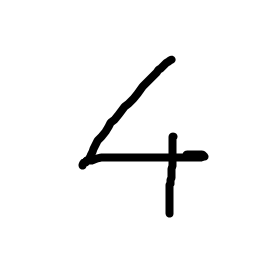
\includegraphics[width=0.2\textwidth]{figures/four.png}
	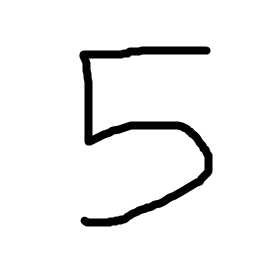
\includegraphics[width=0.2\textwidth]{figures/five.png}
\end{figure}

\subsection{Model Calibration cont.}\label{model-calibration-cont.}

When the parameters of the model we want to calibrate can be expressed
as a function of three variables we can implement a convolutional neural network to work with special images representing our model.

Consider again the Black and Scholes formula for the call options.
Assume you need to calibrate the rate \(r\) and the volatity \(\sigma\)
at the same time. A convolutiona neural network can be trained using
special images which represents \(\mathrm{ttm}, K\) and
\(P_\textrm{call}\).

A black-white image indeed can be interpreted as a map where each pixel
is a pair (\(\mathrm{ttm}, K)\) and the pixel color, an integer between
0 (black) and 255 (white), represents \(P_\textrm{call}\). As in the
previous examples the neural network was classifing the pictures into
digits, now it will assign them to classes identified by \(r, \sigma\)
pairs.

The creation of the training sample is a little more complicated now.
For convenience we will use also a new format to save data image,
\(\tt{numpy}\). This will be done through the corresponding module
simply using the functions \(\tt{save}\) and \(\tt{load}\) to store and
retrieve data. The module \(\tt{PIL}\) (pillow) is instead used to
visualize the images.

First we make the targets.

\begin{tcolorbox}[breakable, size=fbox, boxrule=1pt, pad at break*=1mm,colback=cellbackground, colframe=cellborder]
\begin{Verbatim}[commandchars=\\\{\}]
\PY{k+kn}{import} \PY{n+nn}{numpy} \PY{k}{as} \PY{n+nn}{np}
\PY{k+kn}{from} \PY{n+nn}{finmarkets} \PY{k}{import} \PY{n}{call}
	
\PY{n}{labels} \PY{o}{=} \PY{p}{[}\PY{p}{]}
\PY{n}{rates} \PY{o}{=} \PY{n}{np}\PY{o}{.}\PY{n}{arange}\PY{p}{(}\PY{l+m+mf}{0.01}\PY{p}{,} \PY{l+m+mf}{0.11}\PY{p}{,} \PY{l+m+mf}{0.001}\PY{p}{)}
\PY{n}{vols} \PY{o}{=} \PY{n}{np}\PY{o}{.}\PY{n}{arange}\PY{p}{(}\PY{l+m+mf}{0.1}\PY{p}{,} \PY{l+m+mf}{0.6}\PY{p}{,} \PY{l+m+mf}{0.005}\PY{p}{)}
\PY{k}{for} \PY{n}{i} \PY{o+ow}{in} \PY{n+nb}{range}\PY{p}{(}\PY{n+nb}{len}\PY{p}{(}\PY{n}{vols}\PY{p}{)}\PY{p}{)}\PY{p}{:}
    \PY{k}{for} \PY{n}{j} \PY{o+ow}{in} \PY{n+nb}{range}\PY{p}{(}\PY{n+nb}{len}\PY{p}{(}\PY{n}{rates}\PY{p}{)}\PY{p}{)}\PY{p}{:}
        \PY{n}{labels}\PY{o}{.}\PY{n}{append}\PY{p}{(}\PY{p}{(}\PY{n}{vols}\PY{p}{[}\PY{n}{i}\PY{p}{]}\PY{p}{,} \PY{n}{rates}\PY{p}{[}\PY{n}{j}\PY{p}{]}\PY{p}{)}\PY{p}{)} 
	
\PY{n}{np}\PY{o}{.}\PY{n}{save}\PY{p}{(}\PY{l+s+s2}{\PYZdq{}}\PY{l+s+s2}{2d.np}\PY{l+s+s2}{\PYZdq{}}\PY{p}{,} \PY{n}{labels}\PY{p}{)}
\end{Verbatim}
\end{tcolorbox}

Then we can create the images.

\begin{tcolorbox}[breakable, size=fbox, boxrule=1pt, pad at break*=1mm,colback=cellbackground, colframe=cellborder]
\begin{Verbatim}[commandchars=\\\{\}]
\PY{n}{k} \PY{o}{=} \PY{n}{np}\PY{o}{.}\PY{n}{arange}\PY{p}{(}\PY{l+m+mf}{0.8}\PY{p}{,} \PY{l+m+mf}{1.2}\PY{p}{,} \PY{p}{(}\PY{l+m+mf}{1.2}\PY{o}{\PYZhy{}}\PY{l+m+mf}{0.8}\PY{p}{)}\PY{o}{/}\PY{l+m+mi}{20}\PY{p}{)}
\PY{n}{ttm} \PY{o}{=} \PY{n}{np}\PY{o}{.}\PY{n}{arange}\PY{p}{(}\PY{l+m+mi}{1}\PY{p}{,} \PY{l+m+mi}{5}\PY{p}{,} \PY{l+m+mi}{4}\PY{o}{/}\PY{l+m+mi}{20}\PY{p}{)}
	
\PY{c+c1}{\PYZsh{} for each r, sigma pair}
\PY{c+c1}{\PYZsh{} generate a matrix of prices}
\PY{n}{maximum} \PY{o}{=} \PY{l+m+mi}{0}
\PY{n}{minimum} \PY{o}{=} \PY{n}{np}\PY{o}{.}\PY{n}{inf}
\PY{n}{prices} \PY{o}{=} \PY{p}{[}\PY{p}{]}
\PY{k}{for} \PY{n}{v} \PY{o+ow}{in} \PY{n}{vols}\PY{p}{:}
    \PY{k}{for} \PY{n}{r} \PY{o+ow}{in} \PY{n}{rates}\PY{p}{:}
        \PY{n}{price} \PY{o}{=}  \PY{n}{np}\PY{o}{.}\PY{n}{zeros}\PY{p}{(}\PY{n}{shape}\PY{o}{=}\PY{p}{(}\PY{l+m+mi}{20}\PY{p}{,} \PY{l+m+mi}{20}\PY{p}{)}\PY{p}{)}
        \PY{k}{for} \PY{n}{ik}\PY{p}{,} \PY{n}{kv} \PY{o+ow}{in} \PY{n+nb}{enumerate}\PY{p}{(}\PY{n}{k}\PY{p}{)}\PY{p}{:}
        \PY{k}{for} \PY{n}{it}\PY{p}{,} \PY{n}{t} \PY{o+ow}{in} \PY{n+nb}{enumerate}\PY{p}{(}\PY{n}{ttm}\PY{p}{)}\PY{p}{:}
            \PY{n}{price}\PY{p}{[}\PY{n}{ik}\PY{p}{,} \PY{n}{it}\PY{p}{]} \PY{o}{=} \PY{n}{call}\PY{p}{(}\PY{n}{kv}\PY{p}{,} \PY{n}{r}\PY{p}{,} \PY{n}{v}\PY{p}{,} \PY{n}{t}\PY{p}{)}
            \PY{n}{prices}\PY{o}{.}\PY{n}{append}\PY{p}{(}\PY{n}{price}\PY{p}{)}
            \PY{c+c1}{\PYZsh{} max and min are saved to }
            \PY{c+c1}{\PYZsh{} normalize our matrices}
            \PY{n}{new\PYZus{}max} \PY{o}{=} \PY{n}{np}\PY{o}{.}\PY{n}{max}\PY{p}{(}\PY{n}{price}\PY{p}{)}
            \PY{n}{new\PYZus{}min} \PY{o}{=} \PY{n}{np}\PY{o}{.}\PY{n}{min}\PY{p}{(}\PY{n}{price}\PY{p}{)}
            \PY{k}{if} \PY{n}{new\PYZus{}max} \PY{o}{\PYZgt{}} \PY{n}{maximum}\PY{p}{:}
                \PY{n}{maximum} \PY{o}{=} \PY{n}{new\PYZus{}max}
            \PY{k}{if} \PY{n}{new\PYZus{}min} \PY{o}{\PYZlt{}} \PY{n}{minimum}\PY{p}{:}
                \PY{n}{minimum} \PY{o}{=} \PY{n}{new\PYZus{}min}
	
\PY{k}{for} \PY{n}{ip}\PY{p}{,} \PY{n}{p} \PY{o+ow}{in} \PY{n+nb}{enumerate}\PY{p}{(}\PY{n}{prices}\PY{p}{)}\PY{p}{:}
    \PY{n}{prices}\PY{p}{[}\PY{n}{ip}\PY{p}{]} \PY{o}{=} \PY{n}{np}\PY{o}{.}\PY{n}{interp}\PY{p}{(}\PY{n}{p}\PY{p}{,} \PY{p}{(}\PY{n}{minimum}\PY{p}{,} \PY{n}{maximum}\PY{p}{)}\PY{p}{,} \PY{p}{(}\PY{l+m+mi}{0}\PY{p}{,} \PY{l+m+mi}{1}\PY{p}{)}\PY{p}{)}
	
\PY{n}{np}\PY{o}{.}\PY{n}{save}\PY{p}{(}\PY{l+s+s2}{\PYZdq{}}\PY{l+s+s2}{2d}\PY{l+s+s2}{\PYZdq{}}\PY{p}{,} \PY{n}{prices}\PY{p}{)}
\end{Verbatim}
\end{tcolorbox}

Below an example of the 20x20 images that have been created
\begin{figure}[htb]
\centering

\includegraphics[width=0.4\textwidth]{figures/2d_training_images}
\end{figure}

Then the training is similar to what has been done for the handwritten
digits.

\begin{tcolorbox}[breakable, size=fbox, boxrule=1pt, pad at break*=1mm,colback=cellbackground, colframe=cellborder]
\begin{Verbatim}[commandchars=\\\{\}]
\PY{k+kn}{import} \PY{n+nn}{numpy} \PY{k}{as} \PY{n+nn}{np}
\PY{k+kn}{from} \PY{n+nn}{finnn} \PY{k}{import} \PY{n}{FinNN}
	
\PY{n}{labels} \PY{o}{=} \PY{n}{np}\PY{o}{.}\PY{n}{load}\PY{p}{(}\PY{l+s+s2}{\PYZdq{}}\PY{l+s+s2}{2d\PYZus{}labels.npy}\PY{l+s+s2}{\PYZdq{}}\PY{p}{)}
\PY{n}{images} \PY{o}{=} \PY{n}{np}\PY{o}{.}\PY{n}{load}\PY{p}{(}\PY{l+s+s2}{\PYZdq{}}\PY{l+s+s2}{2d.npy}\PY{l+s+s2}{\PYZdq{}}\PY{p}{)}
	
\PY{n}{trainer} \PY{o}{=} \PY{n}{FinNN}\PY{p}{(}\PY{l+s+s2}{\PYZdq{}}\PY{l+s+s2}{CNN2D}\PY{l+s+s2}{\PYZdq{}}\PY{p}{)}
\PY{n}{trainer}\PY{o}{.}\PY{n}{setData}\PY{p}{(}\PY{n}{images}\PY{p}{,} \PY{n}{labels}\PY{p}{,} \PY{n}{test\PYZus{}size}\PY{o}{=}\PY{l+m+mf}{0.2}\PY{p}{)}
	
\PY{n}{trainer}\PY{o}{.}\PY{n}{addConv2DLayer}\PY{p}{(}\PY{n}{filters}\PY{o}{=}\PY{l+m+mi}{8}\PY{p}{,} \PY{n}{filter\PYZus{}size}\PY{o}{=}\PY{l+m+mi}{10}\PY{p}{,} 
                       \PY{n}{input\PYZus{}shape}\PY{o}{=}\PY{p}{(}\PY{l+m+mi}{20}\PY{p}{,} \PY{l+m+mi}{20}\PY{p}{,} \PY{l+m+mi}{1}\PY{p}{)}\PY{p}{,} \PY{n}{activation}\PY{o}{=}\PY{l+s+s1}{\PYZsq{}}\PY{l+s+s1}{relu}\PY{l+s+s1}{\PYZsq{}}\PY{p}{)}
\PY{n}{trainer}\PY{o}{.}\PY{n}{addFlatten}\PY{p}{(}\PY{p}{)}
\PY{n}{trainer}\PY{o}{.}\PY{n}{addHiddenLayer}\PY{p}{(}\PY{n}{neurons}\PY{o}{=}\PY{l+m+mi}{10}\PY{p}{,} \PY{n}{activation}\PY{o}{=}\PY{l+s+s1}{\PYZsq{}}\PY{l+s+s1}{relu}\PY{l+s+s1}{\PYZsq{}}\PY{p}{)}
\PY{n}{trainer}\PY{o}{.}\PY{n}{addOutputLayer}\PY{p}{(}\PY{n}{outputs}\PY{o}{=}\PY{l+m+mi}{2}\PY{p}{,} \PY{n}{activation}\PY{o}{=}\PY{l+s+s1}{\PYZsq{}}\PY{l+s+s1}{relu}\PY{l+s+s1}{\PYZsq{}}\PY{p}{)}
\PY{n}{trainer}\PY{o}{.}\PY{n}{compileModel}\PY{p}{(}\PY{n}{loss}\PY{o}{=}\PY{l+s+s1}{\PYZsq{}}\PY{l+s+s1}{mse}\PY{l+s+s1}{\PYZsq{}}\PY{p}{,} \PY{n}{opt}\PY{o}{=}\PY{l+s+s1}{\PYZsq{}}\PY{l+s+s1}{adam}\PY{l+s+s1}{\PYZsq{}}\PY{p}{)}
	
\PY{n}{trainer}\PY{o}{.}\PY{n}{fit}\PY{p}{(}\PY{n}{epochs}\PY{o}{=}\PY{l+m+mi}{500}\PY{p}{,}  \PY{n}{verbose}\PY{o}{=}\PY{l+m+mi}{1}\PY{p}{)}
\PY{n}{trainer}\PY{o}{.}\PY{n}{saveModel}\PY{p}{(}\PY{l+s+s2}{\PYZdq{}}\PY{l+s+s2}{2d}\PY{l+s+s2}{\PYZdq{}}\PY{p}{)}
	
\PY{n}{trainer}\PY{o}{.}\PY{n}{evaluate}\PY{p}{(}\PY{p}{)}


Epoch 1/500
8000/8000 [==============================] - 1s 156us/step - loss: 0.0018
Epoch 2/500
8000/8000 [==============================] - 1s 142us/step - loss: 6.2310e-04
...
Epoch 499/500
8000/8000 [==============================] - 2s 194us/step - loss: 1.4921e-06
Epoch 500/500
8000/8000 [==============================] - 2s 193us/step - loss: 1.4413e-06

8000/8000 [==============================] - 1s 65us/step
Training: 1.1013161047230825e-05
2000/2000 [==============================] - 0s 70us/step
Test: 1.116331470257137e-05
\end{Verbatim}
\end{tcolorbox}

At this point you should present to the trained CNN the prices of call
referring to the same underlying in the pictorial form shown before and
the in response it will give you the risk-free rate and the underlying
volatility.

\begin{tcolorbox}[breakable, size=fbox, boxrule=1pt, pad at break*=1mm,colback=cellbackground, colframe=cellborder]
\begin{Verbatim}[commandchars=\\\{\}]
\PY{k}{for} \PY{n}{i} \PY{o+ow}{in} \PY{n+nb}{range}\PY{p}{(}\PY{l+m+mi}{5}\PY{p}{)}\PY{p}{:}
    \PY{n+nb}{print} \PY{p}{(}\PY{n}{trainer}\PY{o}{.}\PY{n}{predict}\PY{p}{(}\PY{n}{trainer}\PY{o}{.}\PY{n}{x\PYZus{}test}\PY{p}{[}\PY{n}{i}\PY{p}{:}\PY{n}{i}\PY{o}{+}\PY{l+m+mi}{1}\PY{p}{]}\PY{p}{)}\PY{p}{)}

[[0.3825101  0.09229672]]
[[0.4056808  0.02232919]]
[[0.47402808 0.05630913]]
[[0.2851617  0.05214534]]
[[0.17245176 0.08815573]]
\end{Verbatim}
\end{tcolorbox}

\section{Technical Analysis}\label{technical-analysis}

In finance, \emph{technical analysis} is a security analysis discipline
for forecasting the direction of prices through the study of past market
data, primarily price and volume. Essentially the analyst looks for
particular patterns in the price time series that are \emph{known} to
develop in predictable ways to take profit of it, Fig.~\ref{fig:tech_ana} shows two
os such patterns.

\begin{figure}[htb]
	\centering
	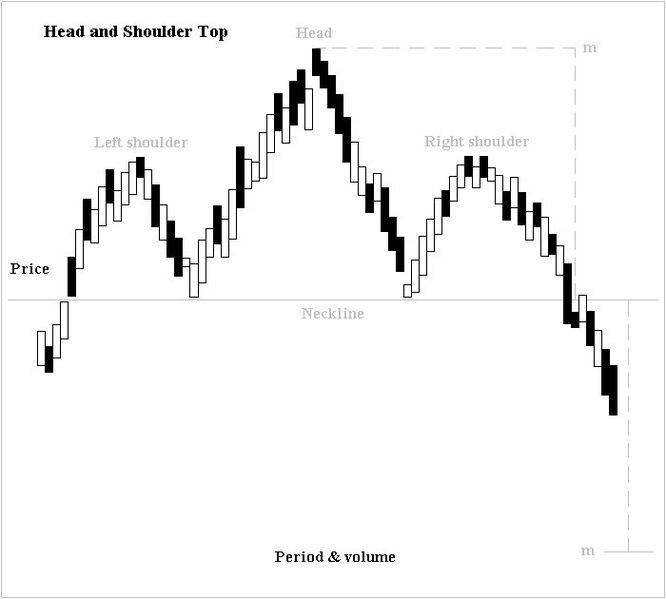
\includegraphics[width=0.4\linewidth]{figures/H_and_s_top_new.jpg}\qquad
	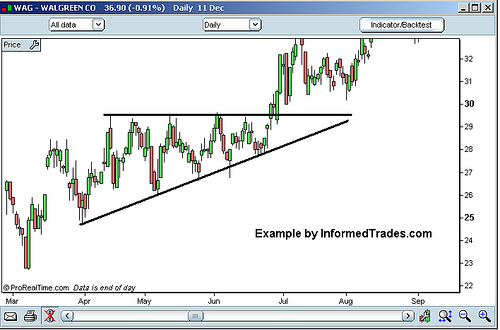
\includegraphics[width=0.4\linewidth]{figures/Triangle-ascending.jpg}
	\caption{Examples of patterns in real time series, head and shoulder (left), triangle (right).}
        \label{fig:tech_ana}
\end{figure}

As you may imagine we will try to develop a CNN (like in the handwriting
case) capable of classifying features in time series to be used in a
technical analysis (this is much faster than having somebody looking at
thousands of time series by eye\ldots{}).

I have generated myself the training set simulating 21600 time series
(1/3 with head and shoulder patter, 1/3 with triangle pattern and 1/3
with no pattern), see Fig~\ref{fig:no_pattern} to~\ref{fig:triangle}.
\emph{To make the training easier the features have been exagerated.}

\begin{figure}
	\centering
	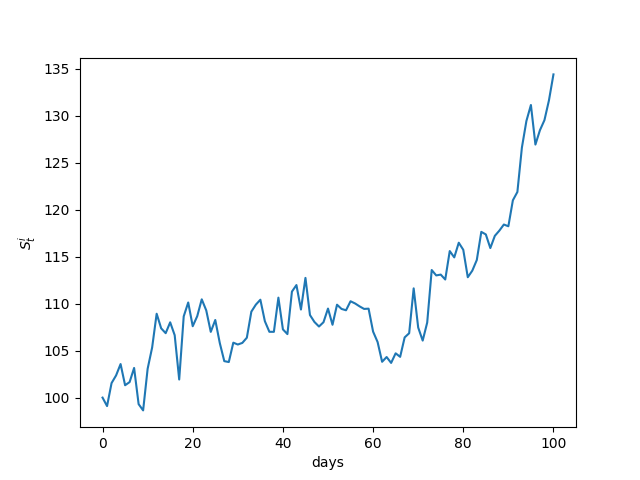
\includegraphics[width=0.5\linewidth]{figures/image_1.png}
	\caption{An example of training image with no pattern.}
        \label{fig:no_pattern}
\end{figure}

\begin{figure}
	\centering
	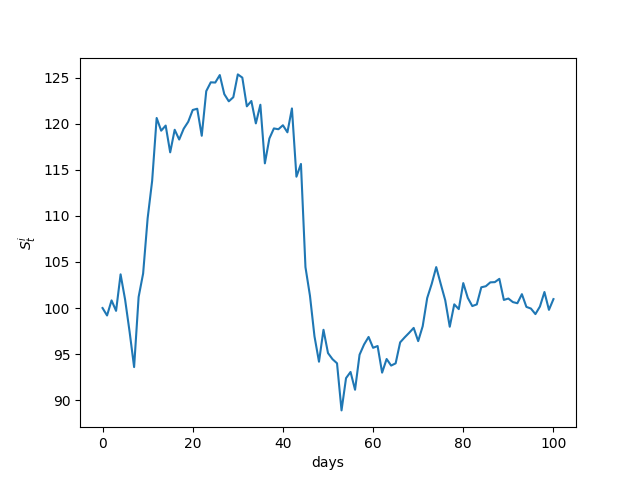
\includegraphics[width=0.5\linewidth]{figures/image_2.png}
	\caption{An example of training image with \emph{head and shoulder} pattern.}
        \label{fig:head_and_shoulder}
\end{figure}

\begin{figure}
	\centering
	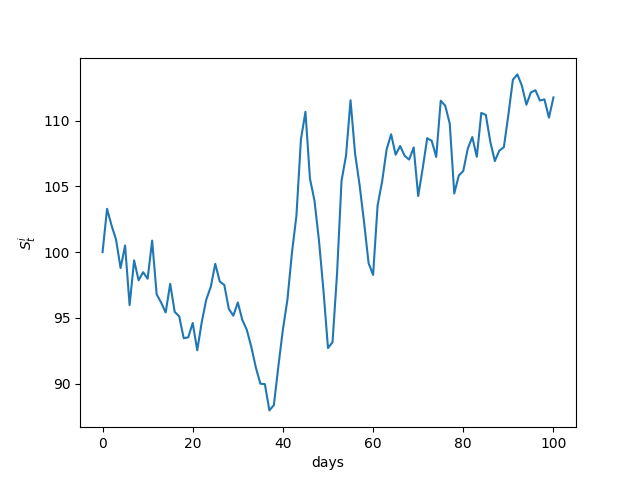
\includegraphics[width=0.5\linewidth]{figures/image_0.png}
	\caption{An example of training image with \emph{triangle} pattern.}
        \label{fig:triangle}
\end{figure}

\begin{tcolorbox}[breakable, size=fbox, boxrule=1pt, pad at break*=1mm,colback=cellbackground, colframe=cellborder]
\begin{Verbatim}[commandchars=\\\{\}]
\PY{k+kn}{import} \PY{n+nn}{numpy} \PY{k}{as} \PY{n+nn}{np}
\PY{k+kn}{from} \PY{n+nn}{finnn} \PY{k}{import} \PY{n}{FinNN}
	
\PY{n}{train\PYZus{}labels} \PY{o}{=} \PY{n}{np}\PY{o}{.}\PY{n}{load}\PY{p}{(}\PY{l+s+s2}{\PYZdq{}}\PY{l+s+s2}{training\PYZus{}techana\PYZus{}labels.npy}\PY{l+s+s2}{\PYZdq{}}\PY{p}{)}
\PY{n}{train\PYZus{}images} \PY{o}{=} \PY{n}{np}\PY{o}{.}\PY{n}{load}\PY{p}{(}\PY{l+s+s2}{\PYZdq{}}\PY{l+s+s2}{training\PYZus{}techana\PYZus{}images.npy}\PY{l+s+s2}{\PYZdq{}}\PY{p}{)}
	
\PY{n}{trainer} \PY{o}{=} \PY{n}{FinNN}\PY{p}{(}\PY{l+s+s2}{\PYZdq{}}\PY{l+s+s2}{CNN1D}\PY{l+s+s2}{\PYZdq{}}\PY{p}{)}
\PY{n}{trainer}\PY{o}{.}\PY{n}{setData}\PY{p}{(}\PY{n}{train\PYZus{}images}\PY{p}{,} \PY{n}{train\PYZus{}labels}\PY{p}{)}
	
\PY{c+c1}{\PYZsh{} define the CNN }
\PY{n}{trainer}\PY{o}{.}\PY{n}{addConv1DInputLayer}\PY{p}{(}\PY{n}{filters}\PY{o}{=}\PY{l+m+mi}{80}\PY{p}{,} \PY{n}{filter\PYZus{}size}\PY{o}{=}\PY{l+m+mi}{20}\PY{p}{,} 
                            \PY{n}{input\PYZus{}size}\PY{o}{=}\PY{p}{(}\PY{l+m+mi}{101}\PY{p}{,} \PY{l+m+mi}{1}\PY{p}{)}\PY{p}{)}
\PY{n}{trainer}\PY{o}{.}\PY{n}{addConv1DLayer}\PY{p}{(}\PY{n}{filters}\PY{o}{=}\PY{l+m+mi}{80}\PY{p}{,} \PY{n}{filter\PYZus{}size}\PY{o}{=}\PY{l+m+mi}{15}\PY{p}{)}
\PY{n}{trainer}\PY{o}{.}\PY{n}{addMaxPooling1D}\PY{p}{(}\PY{l+m+mi}{3}\PY{p}{)}
\PY{n}{trainer}\PY{o}{.}\PY{n}{addConv1DLayer}\PY{p}{(}\PY{n}{filters}\PY{o}{=}\PY{l+m+mi}{100}\PY{p}{,} \PY{n}{filter\PYZus{}size}\PY{o}{=}\PY{l+m+mi}{10}\PY{p}{)}
\PY{n}{trainer}\PY{o}{.}\PY{n}{addConv1DLayer}\PY{p}{(}\PY{n}{filters}\PY{o}{=}\PY{l+m+mi}{100}\PY{p}{,} \PY{n}{filter\PYZus{}size}\PY{o}{=}\PY{l+m+mi}{5}\PY{p}{)}
\PY{n}{trainer}\PY{o}{.}\PY{n}{addGlobalAveragePooling1D}\PY{p}{(}\PY{p}{)}
\PY{n}{trainer}\PY{o}{.}\PY{n}{addDropout}\PY{p}{(}\PY{l+m+mf}{0.5}\PY{p}{)}
\PY{n}{trainer}\PY{o}{.}\PY{n}{addCNNOutputLayer}\PY{p}{(}\PY{n}{outputs}\PY{o}{=}\PY{l+m+mi}{3}\PY{p}{)}
\PY{n}{trainer}\PY{o}{.}\PY{n}{compileModel}\PY{p}{(}\PY{n}{loss}\PY{o}{=}\PY{l+s+s1}{\PYZsq{}}\PY{l+s+s1}{categorical\PYZus{}crossentropy}\PY{l+s+s1}{\PYZsq{}}\PY{p}{,} \PY{n}{opt}\PY{o}{=}\PY{l+s+s1}{\PYZsq{}}\PY{l+s+s1}{adam}\PY{l+s+s1}{\PYZsq{}}\PY{p}{)}
	
\PY{n}{trainer}\PY{o}{.}\PY{n}{fit}\PY{p}{(}\PY{n}{epochs}\PY{o}{=}\PY{l+m+mi}{80}\PY{p}{)}
	
\PY{n}{trainer}\PY{o}{.}\PY{n}{saveModel}\PY{p}{(}\PY{l+s+s1}{\PYZsq{}}\PY{l+s+s1}{techana}\PY{l+s+s1}{\PYZsq{}}\PY{p}{)}

Epoch 1/80
- 23s 1ms/step - loss: 0.6773
Epoch 2/80
- 23s 1ms/step - loss: 0.5421
...
Epoch 79/80
- 23s - loss: 0.0737
Epoch 80/80
- 23s - loss: 0.0692
\end{Verbatim}
\end{tcolorbox}

\begin{tcolorbox}[breakable, size=fbox, boxrule=1pt, pad at break*=1mm,colback=cream, colframe=cellborder]
\subsubsection{Again for the Most Curious}\label{again-for-the-most-curious}

Large neural nets trained on relatively small datasets can overfit the
training data.

This has the effect of the model learning the statistical noise in the
training data, which results in poor performance when the model is
evaluated on new data, e.g.~a test dataset.

One approach to reduce overfitting is to fit all possible different
neural networks on the same dataset and to average the predictions from
each model. This is not feasible in practice, and can be approximated
using a small collection of different models, called an ensemble. A
problem even with the ensemble approximation is that it requires
multiple models to be fit and stored, which can be a challenge if the
models are large, requiring days or weeks to train and tune.

\emph{Dropout} is a regularization method that approximates training a
large number of neural networks with different architectures in
parallel.

During training, some number of layer outputs are randomly ignored or
\emph{dropped out}. This has the effect of making the layer look-like
and be treated-like a layer with a different number of nodes and
connectivity to the prior layer. In effect, each update to a layer
during training is performed with a different ``view'' of the configured
layer.

Even if the it may seems counter intuitive (better training when
switching off nodes) indeed dropout breaks-up situations where network
layers co-adapt to correct mistakes from prior layers, in turn making
the model more robust.
\end{tcolorbox}

To test the perfomance I wanted to simulate a real case scenario where
the time series are analyzed in real-time in order to predict as soon as
possible a particular pattern and take advantage of the prediction.

To do so I have created a longer time series (i.e.~more time points) and
passed as input to the CNN sliding time windows to simulate the
evolution of the time series. So if for example the time series is made
of 100 points, I presented to the network first the points between
\([0, 80]\), then \([1, 81]\), \([2, 82]\) and so on simulating new real
time data incoming. The goal was to check when the neural network was
capable of predicting the incoming pattern. Figure~\ref{fig:frame_simulation}
is showing the "temporal frames" that have been presented to the CNN for predicting possible incoming patterns.

\begin{figure}
	\centering
	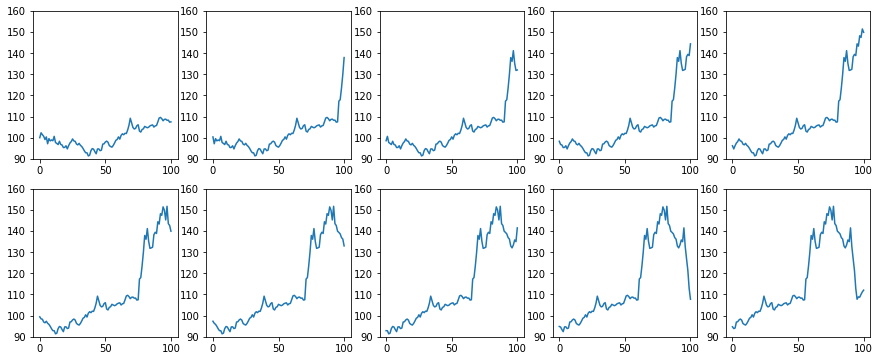
\includegraphics[width=\textwidth]{figures/tech_ana_frames.png}
	\caption{Ten frames simulating closing price date incoming in real time. The CNN was tested to check if and when it would have been able to detect any pattern in data.}
	\label{fig:frame_simulation}
\end{figure}


\begin{tcolorbox}[breakable, size=fbox, boxrule=1pt, pad at break*=1mm,colback=cellbackground, colframe=cellborder]
\begin{Verbatim}[commandchars=\\\{\}]
\PY{n}{test\PYZus{}images} \PY{o}{=} \PY{n}{np}\PY{o}{.}\PY{n}{load}\PY{p}{(}\PY{l+s+s2}{\PYZdq{}}\PY{l+s+s2}{testing\PYZus{}techana\PYZus{}frames.npy}\PY{l+s+s2}{\PYZdq{}}\PY{p}{)}
\PY{n}{trainer}\PY{o}{.}\PY{n}{loadModel}\PY{p}{(}\PY{l+s+s2}{\PYZdq{}}\PY{l+s+s2}{techana}\PY{l+s+s2}{\PYZdq{}}\PY{p}{)}
	
\PY{n}{predictions} \PY{o}{=} \PY{n}{trainer}\PY{o}{.}\PY{n}{predict}\PY{p}{(}\PY{n}{test\PYZus{}images}\PY{p}{)}
\PY{k}{for} \PY{n}{i} \PY{o+ow}{in} \PY{n+nb}{range}\PY{p}{(}\PY{n+nb}{len}\PY{p}{(}\PY{n}{predictions}\PY{p}{)}\PY{p}{)}\PY{p}{:}
    \PY{n+nb}{print} \PY{p}{(}\PY{n}{np}\PY{o}{.}\PY{n}{argmax}\PY{p}{(}\PY{n}{predictions}\PY{p}{[}\PY{n}{i}\PY{p}{]}\PY{p}{)}\PY{p}{,} \PY{p}{[}\PY{l+s+s2}{\PYZdq{}}\PY{l+s+si}{\PYZob{}:.3f\PYZcb{}}\PY{l+s+s2}{\PYZdq{}}\PY{o}{.}\PY{n}{format}\PY{p}{(}\PY{n}{p}\PY{p}{)} \PY{k}{for} \PY{n}{p} \PY{o+ow}{in} \PY{n}{predictions}\PY{p}{[}\PY{n}{i}\PY{p}{]}\PY{p}{]}\PY{p}{)}

0 ['0.942', '0.000', '0.058']
0 ['0.970', '0.000', '0.030']
0 ['1.000', '0.000', '0.000']
0 ['0.999', '0.001', '0.000']
0 ['0.784', '0.216', '0.000']
1 ['0.000', '1.000', '0.000']
1 ['0.000', '1.000', '0.000']
1 ['0.000', '1.000', '0.000']
1 ['0.000', '1.000', '0.000']
1 ['0.000', '1.000', '0.000']
\end{Verbatim}
\end{tcolorbox}

So at the 6th sample the CNN start recognizing the \emph{head and
shoulder} pattern in the price evolution.


https://arxiv.org/abs/1705.08807
https://www.deeplearningbook.org/

	arXiv:2101.09957 Activation Functions in Artificial Neural Networks: A Systematic Overview
	Johannes Lederer
	
	